\documentclass[english, a4paper, 12pt]{article}

%:Preamble
%:	Packages
\usepackage[bookmarks, colorlinks=true, allcolors=blue, pagebackref=true, hyperfootnotes=false]{hyperref}
\usepackage[eng]{felipito}
\usepackage[round]{natbib}

%:	Graphics path
\graphicspath{{./Graphics/}}

%:	Dimensions and spacing: A4 -> 595x842
\usepackage[margin=2cm]{geometry}
\spacing{1.2}

%:	Epigraph settings
\setlength{\epigraphwidth}{0.59\textwidth}

%:	Title page content
\author{Felipe Del Canto M.}
\title{Aggregate problems require aggregate solutions? \\ When heterogeneity is expendable}
\date{\today}

%:Document
\begin{document}

%:	Title page 
\maketitle
\thispagestyle{empty}

%:	Abstract

\vfill
\epigraph{(...) all models are approximations. Essentially, all models are wrong, but some are useful. However, %
the approximate nature of the model must always be borne in mind.}{\textit{Empirical Model-Building and Response Surfaces (1987)} \\ \textsc{George Box and Norman Draper}}

\vfill
{\abstract Aggregation is a tool used to reduce the complexity of economic models in order to draw more clear and succinct conclusions or simplify analyses. As any approximation, its use may be accompanied with errors researchers may not be willing to tolerate if they become aware of them. In this work I present how these errors appear using aggregation across goods and across consumers. To this end, I consider aggregation as a means to approximate probability distributions over parameters. Using this approach, I show ways to bound approximation errors by tailoring the parameters of the model. Further, I briefly discuss a methodology to study the goodness-of-fit of aggregate models in more general settings.}
\vfill

\spacing{1.5}

\newpage
%%%	Introduction	%%%
\section{Introduction}

%:	General importance of models in science and in economics. The assumptions problem and measuring GoF
Every model in science is by definition a simplified reality. On the bright side, abstracting from the complexity of the real world has allowed society to understand the sometimes subtle mechanisms that rule nature and human behavior. This does not mean that a model is useful for every purpose. Evidently, whilst some of them can illustrate certain dynamics of the real world very clearly, approximation in itself may carry errors that harm future predictions. The previous comment points directly to the question of which model is the most useful for a given problem. In particular, when the answer is \textit{many} the modeler needs to make a choice based on the results she expects to highlight and the channels she wants to study. The dilemma is by no means alien to the field of economics. When describing an economy, the researcher faces several different assumptions that shape the complexity of the model. Although some of them may be made for feasibility reasons (e.g., because a highly detailed model cannot be solved or simulated or because data is not available to calibrate it) there may be others that serve a transparency purpose, that is, they intend to highlight the most important results without dwelling on the unnecessary details. Consequently, in the process of constructing a model, the investigator may choose to follow the Occam's Razor principle: among the models that are consistent with the evidence, choose the one that makes the fewest assumptions. This criterion implies that the measure of a (correct) model is its complexity. However, as Milton Friedman said, ``The ultimate goal of a positive science is the development of a `theory' or, `hypothesis' that yields valid and meaningful (...) predictions about phenomena not yet observed'' and thus ``Its performance is to be judged by the precision, scope, and conformity with experience of the predictions it yields''.\footnote{\,\cite{FriedmanPositive}.} Hence, in evaluating the validity of a theory, the robustness of its conclusions should be of critical importance.

%:	Related literature that supports relevance
Different strands in the economic literature have studied when predictions derived from a model are robust to different specifications. In \cite{SuttonMarketStruct}, the author discusses which mechanisms in the context of industrial organization still hold in conditions outside the classical models of, for example, Cournot and Bertrand. A similar motivation can be found in \cite{Morris97}, where they study how sensitive game theory conclusions are to the assumption of common knowledge of payoffs in a game. The interest in robustness in the context of mechanism design can be also found in \cite{Morris2011}. An interesting approach is the one in \cite{Basu97} where the authors try to estimate discrepancies due to ``aggregation effects'' when considering a model with a representative firm and one where heterogeneous effects are considered. Similarly, in \cite{SchoolAggregation} the authors try to reconcile contradictory results in the literature on estimating the value added by schools arguing an important role of aggregation in the magnitude of omitted variable bias, which can in principle invalidate previous estimations. Related to this literature there is a concern with models that make use of aggregated data. Different authors have studied what is called ``aggregation bias'' arguing that these models hide important mechanisms that could explain these differences.\footnote{\,See, for example \cite{Agg1, Agg2, Agg3, Agg4}.} All in all, different authors have tried to untangle the differences between predictions and realizations by appealing to the goodness-of-fit of the models used to produce such estimations. In the cases where the deviations are substantial, a revision to the model must be made.

%:	Representative agent model problems (critics?)
As an example, consider the case of the representative agent model. The assumption that there is only one consumer in the economy is useful and has been key to understand important qualitative results, especially in macroeconomics. Nevertheless, employing this model to predict future realizations of certain key variables such as aggregate demand or marginal propensity to consume (MPC) may be inaccurate if heterogeneity effects are in place. In other words, there is a shadow price in the approximation (which the investigator could be willing to pay or not) if she wishes to use the model for another, more quantitative-driven purpose. This point is made clearly in \cite{CarrollRequiem} in the context of the buffer-stock model: ``Representative-agent models are typically calibrated to match an aggregate wealth-to-income ratio'' but ``the typical household’s wealth is much smaller than the wealth of such a representative agent (...), this would lead one to expect that the behavior of the median household may not resemble the behavior of a representative agent with a wealth-to-income ratio similar to the aggregate ratio''. The evidence quickly back this view up: while the annual MPC predicted by the representative agent model is about 0.04, many empirical analyses estimate this parameter to lie between 0.2 and 0.5.\footnote{\,\cite{CarrollRequiem}.} 

%:	Aggregation in particular
The aforementioned model is a particular case of a common practice in economics: aggregation. The other canonical example of its use is aggregation across goods, where instead of describing the myriad of goods available in an economy they are grouped into one or more categories. Regarding these two implementations, previous theoretical literature focused on one side of the problem: When it is possible to carry out this practice and describe precisely the same economy. In the case of the representative agent, the necessary and sufficient condition is that the indirect utility function of every consumer has the Gorman form.\footnote{\,\cite{Gorman53}.} When aggregation is applied to goods, the answer has been more elusive but two results have arisen. First, the Hicks-Leontief (composite commodity) theorem allows aggregation if relative prices are constant in the group of goods that are to be bundled.\footnote{\,\cite{Leontief36, HicksBook}.} A somewhat weaker requirement is proposed by \cite{Lewbel96}: bundling is feasible if all group relative prices are independent of price indexes and income. The second answer states that grouping some goods is allowed if preferences between them are ``independent'' of the remaining goods present in the economy.\footnote{\,See for example \cite{GormanSeparability}.} 

%:	Main idea using aggregation
For the two kinds of aggregation mentioned before, the conditions for them to hold are highly restrictive and not typically met in econometric or theoretical applications. As mentioned previously, the literature has assumed (disregarding these conditions) exact aggregation of both types in constructing models and making econometric estimations and this practice comes at a price. As was stated in the preceding discussion, the validity of these models is directly attached to the size of such cost. If the question an investigator is seeking to answer allows the use of aggregate models without incurring in a severe deviation from predictions, then not having exact aggregation is of minor importance. In other words, compliance of the conditions for aggregation is not a problem as long as the parameters of the simplified model are calibrated in such a way that the estimation error is below some tolerance predefined by the modeler. Hence, understanding and quantifying these differences is crucial in determining and measuring the goodness-of-fit of these models. Consequently, and in contrast with some of the articles mentioned earlier, in this work I intend to give a theoretical look at how these deviations appear using simple models and understand how a researcher might limit them. To this end, the main insight I employ is that aggregation is trading off heterogeneity for simplicity and from here is where errors make their appearance. Explicitly, I model heterogeneity as a probability distribution over the relevant parameters of the economy, where relevance is understood depending on the research question asked. In that context, aggregation is replacing the distribution of unknown relevant parameters by a Dirac distribution centered at a point chosen by the modeler. Thus, the approximation error is closely related to the nature of the original and the approximate distributions, specifically to some finite set of moments of them.

%:	Main idea in general
Reformulating the problem in this manner has consequences beyond the particular case of aggregate models. Diversity appears naturally in many applications and hence modeling it as a distribution allows the investigator to define the problem in more clearer terms. After determining the relevant sources of heterogeneity in the specific context, only remains to pick an appropriate measure of the error that, conditional on the precision desired, narrows the range of distributions available for replacement. The advantage of this line of thinking is that the optimal metric can be created following the Friedman guidelines mentioned above. This way, models are evaluated under the scope of the quality of their predictions and not on their complexity. Moreover, the methodology proposed here serves also as a decision rule, leaving arbitrary choices outside the modeling process.

%:	Index
The rest of the paper proceeds as follows. To motivate the subsequent discussion, in \Cref{sec:PrevResults} I summarize the problems and previous results regarding conditions under which aggregation is permitted. Then, I present three settings to illustrate how approximation errors appear when using aggregate models to estimate future economic variables. First, in \Cref{sec:RepAg}, I propose a representative agent model in the context of aggregate demand estimation. Second, in \Cref{sec:CarrollAgg}, I study a different setting with a representative agent model but where the objective is to estimate the MPC. The third model, in \Cref{sec:MixedAgg}, mixes the two canonical types of aggregation by presenting an economy composed of several individuals consuming various goods, where good aggregation takes a different form for each of the agents. Finally, in \Cref{sec:Conclusion} I discuss how to generalize the problem of heterogeneity approximation, detailing the precise methodology that must be followed in order to reformulate it.

%%%	Previous results in aggregation	%%%
\section{Previous results in aggregation} \label{sec:PrevResults}
The economic literature has recognized two forms of aggregation that are usually taught in microeconomics courses around the world. First, the problem of consumer aggregation or the representative agent model seeks to describe the aggregate demand of a multi-person economy by focusing only on the aggregate determinants of demand (e.g., the aggregate income), as opposed to the distribution of such variables. The second class of aggregation focuses on describing demands for categories of goods without distinguishing the individual consumption of each element in the group. I refer to this last problem as the ``Hicksian aggregation problem''.

Both kinds of aggregation are widely used in economic models. The representative consumer was a salient feature of macroeconomic models, like the ones developed by Robert Lucas in 1978 to study asset prices and by Kydland and Prescott in 1982, that began the theory of real business cycles.\footnote{\,See \cite{Lucas78} and \cite{KyPr82}.} These authors also make use of aggregation across goods by employing a two-good model, although this feature has also been widely used to study the behavior of savings (in particular, precautionary savings during the life cycle) or consumption dynamics.\footnote{\,See \cite{Carroll92}, \cite{GourinchasParker02}, \cite{GulPesendorfer04}, \cite{ParkerPreston05} for some examples.} Empirical studies also make use of both forms of aggregation. Some of them assume all consumers are equal which is an example of consumer aggregation and others overcome problems in the data (e.g., availability or comprehensiveness) by stating that agents choose consumption on the category and not on individual goods.\footnote{\,See \cite{KaplanViolante14}, \cite{BergerVavra15}, \cite{KanPengWang17}, \cite{FagerengGuisoPistaferri17} for some examples.}

In what follows I formally describe the problems about aggregation the early literature tried to answer. These questions aimed at ing conditions that ensured aggregation did an exact fit of an heterogeneous model. In order to describe both problems I rely heavily on \cite{VarianBook}.

	%%	The representative agent problem	%%
\subsection{The representative agent problem} \label{ssec:RepAgent}
Consider an economy composed by $n$ consumers indexed by $i = 1, \ldots, n$. Their demand functions of the $k$ goods in the economy are summarized in the vector $\mathbf{x}_{i}(\mathbf{p}, y_{i})$, where $\mathbf{p}$ is the price vector of the goods and $y_{i}$ is the income of agent $i$. The aggregate demand vector is defined by
	\begin{equation} \label{eq:aggdemand1}
		\mathbf{X}(\mathbf{p}, y_{1}, \ldots, y_{n}) = \sum_{i=1}^{n} \mathbf{x}_{i}(\mathbf{p},y_{i}).
	\end{equation}

The question that automatically arises is: Can this aggregate demand function be regarded as the one generated by a single (or ``representative'') consumer? According to \eqref{eq:aggdemand1}, the previous question is equivalent to looking for conditions under which $\mathbf{X}$ does not depend on the distribution but on the aggregate income
	$$Y := \sum_{i=1}^{n} y_{i}.$$
The definitive answer to this problem came with \cite{Gorman53}. According to his result, $\mathbf{X}$ is a function of $Y$ if and only if for every $i \in \{1,\ldots,n\}$ the indirect utility function has the Gorman form
	$$v_{i}(\mathbf{p}, y_{i}) = a_{i}(\mathbf{p}) + b(\mathbf{p})y_{i},$$ 
where $a_{i}, b$ are functions that must only depend on $\mathbf{p}$ and $b$ has to be the same across consumers. This functional requirement is somewhat restrictive but at least two particular examples are worth mentioning: homothetic and quasilinear utility functions. For the first, the indirect utility functions is
	\begin{equation} \label{eq:homotheticindirect}
		v(\mathbf{p}, y) = b(\mathbf{p})y,
	\end{equation}
whereas for the second
	$$v(\mathbf{p}, y) = a(\mathbf{p}) + y.$$
Both examples clearly have the Gorman form. However, some homothetic functions can differ in the function $v$ between consumers and thus aggregation is not possible. As an example, for $k = 2$, an economy of consumers with Cobb-Douglas utility functions
	$$u(x_{1}, x_{2}) = x_{1}^{\alpha_{i}}x_{2}^{1-\alpha_{i}},$$
where at least two $\alpha_{i}$ are different does not allow aggregation. In this case the function $v(\mathbf{p})$ in \eqref{eq:homotheticindirect} is different among individuals and the Gorman form is not present.

Observe that main objective of the representative agent problem is to find an alternative model that is completely coherent with the original. That is, this new, simpler model has to describe the exactly same economy as the disaggregate one. Backing this task is the idea that models should fit exactly in the context they intend to describe. However, since the original model is an approximation by itself, a more consistent approach is to consider the second fit as an additional layer of estimation and thus weigh its suitability in terms of the accuracy loss and the potential additional insight obtained.

	%%	Hicksian aggregation	%%
\subsection{Hicksian aggregation problem} \label{ssec:HicksAgg}
For this problem consider the following setting. Assume the consumption vector of some agent is divided in two bundles $(\mathbf{x}, \mathbf{z})$. Accordingly, the price vector is separated into $(\mathbf{p}, \mathbf{q})$. Thus, if the utility function of the consumer is $u$, then the demand for the $\mathbf{x}$ goods is
	\begin{equation} \label{eq:hickdisprob}
		\probop[s.t.]{\mathbf{x}(\mathbf{p}, \mathbf{q}, y) = \argmax_{\mathbf{x}, \mathbf{z}}}{u(\mathbf{x}, \mathbf{z})}
					{&	\mathbf{px} + \mathbf{qz} = y.}
	\end{equation}

In numerous models, there is no interest in the consumption of each of the $\mathbf{x}$-goods but only in the demand for the bundle (e.g., focus on expenditure in savings against expenditure in different financial instruments). Hence, the Hicksian aggregation problem is finding conditions under which this approximation can be made without losing information. This implies finding a quantity index $X = g(\mathbf{x})$, a price index $P = f(\mathbf{p})$ and a new utility function $U(X, \mathbf{z})$ such that the solution
	 \begin{equation} \label{eq:hickaggprob}
		\probop[s.t.]{X(P, \mathbf{q}, y) = \argmax_{X, \mathbf{z}}}{U(X, \mathbf{z})}
					{&	PX + \mathbf{qz} = y.}
	\end{equation}
satisfies
	$$X(f(\mathbf{p}), \mathbf{q}, y) = g(\mathbf{x}(\mathbf{p}, \mathbf{q}, y)).$$
In other words, the objective is to find an alternative model that is coherent with the original. This brings out again the discussion at the end of the preceding section: Aggregation can be regarded as a second layer of approximation and thus be pondered in terms of its benefits and costs. In this particular setting, the nature of the approximation is different, but the essence of simplifying the world remains.

At least two situations exist under which these alternative models can be found: functional and Hicksian separability. In the first, assume that the preference relation represented by $u$ has the following ``independence'' property
	\begin{equation} \label{eq:indepPref}
		(\mathbf{x}, \mathbf{z}) \succ (\mathbf{x}', \mathbf{z}) 
			\Longleftrightarrow
		(\mathbf{x}, \mathbf{z}') \succ (\mathbf{x}', \mathbf{z}') \qquad \paratodo \mathbf{x}, \mathbf{x}', \mathbf{z}, \mathbf{z}'.
	\end{equation}
This independence property implies that there exists a function $v$ such that
	$$u(\mathbf{x}, \mathbf{z}) = U(v(\mathbf{x}), \mathbf{z}),$$
where $U(v,\mathbf{z})$ is increasing in $v$. In this case, the consumer values consumption of $\mathbf{x}$ only through $v$. For example, consider $\mathbf{x}$ to be different types of food. Independence in this context could manifest if the agent only values the amount of calories she gets from $\mathbf{x}$. In that situation, all kinds of food are valued differently according to the amount of calories per unit each of them give but the consumer only cares about the total caloric intake. The previous example suggests a particularity of this type of separability. Following the same nomenclature: The consumer chooses the amount of calories and the total amount to spend on food first and then she decides the individual consumption of each kind of food. Models that show this feature are often referred to as hierarchical consumption models.

By calling $m_{\mathbf{x}} := \mathbf{p}\cdot \mathbf{x}(\mathbf{p}, \mathbf{q}, y)$, it can be shown that the following equality holds
	$$\probop[s.t.]{\mathbf{x}(\mathbf{p}, \mathbf{q}, y) = \argmax_{\mathbf{x}}}{v(\mathbf{x})}
					{&	\mathbf{px} = m_{\mathbf{x}}.}$$
Thus, if $e(\mathbf{p}, v)$ is the expenditure function of the previous problem, then
	$$	\probop[s.t.]{v(\mathbf{x}(\mathbf{p}, \mathbf{q}, y)) = \argmax_{v, \mathbf{z}}}{U(v, \mathbf{z})}
				{&	e(\mathbf{p}, v) + \mathbf{qz} = y.}
	$$
However, note that the latter problem does not have the same structure as \eqref{eq:hickaggprob}. This only happens if $v$ has a particular structure such that 
	$$e(\mathbf{p}, v) = e(\mathbf{p})v.$$
This property holds if, for example, $v$ is homothetic and thus the Cobb-Douglas utility function is an example in which this kind of aggregation is admissible. The previous discussion shows that under functional separability this consumption model is hierarchical.

On the other hand, Hicksian separability is present in the following situation. Assume that $\mathbf{p} = t\mathbf{p}_{0}$, where $t$ is a scalar and $\mathbf{p}_{0}$ is a fixed price vector. Letting $P := t$ and $X := \mathbf{p}_{0}\mathbf{x}$, define the following indirect utility function
	$$	\probop[s.t.]{V(P, \mathbf{q}, y) = \argmax_{\mathbf{x}, \mathbf{z}}}{u(\mathbf{x}, \mathbf{z})}
				{&	P\mathbf{p}_{0}\mathbf{x} + \mathbf{qz} = y.}
	$$
The solution $U$ of the dual problem
	$$	\probop[s.t.]{U(X, \mathbf{z}) = \argmin_{P, \mathbf{q}}}{V(P, \mathbf{q},y)}
				{&	PX + \mathbf{qz} = y,}
	$$
by definition satisfies
	$$	\probop[s.t.]{V(P, \mathbf{q}, y) = \argmax_{X, \mathbf{z}}}{U(X, \mathbf{z})}
				{&	PX + \mathbf{qz} = y.}
	$$
showing that aggregation is possible with $g(\mathbf{x}) = \mathbf{p}_{0}\mathbf{x}$ and $f(\mathbf{p}) = t$. This result was both presented by \cite{Leontief36} and \cite{HicksBook} and thus has been called the Hicks-Leontief theorem. As was the case with functional separability, note that the theorem presents sufficient but not necessary conditions to find the functions $g$, $f$ and $U$. In his work, \cite{Lewbel96} relaxes the assumptions of the Hicks-Leontief theorem by not asking for constant relative prices through time but instead for them to be independent of both the price index and income. In terms of data analysis, the generalized composite commodity theorem of Lewbel does not ask for a correlation of one between the price of the $\mathbf{x}$-goods and their index.

One of the most common applications of good aggregation under Hicksian separability assumptions are two-good models. Here, the interest is in the demand for one good while bundling all the other goods in only one category. These kind of models are frequently used in the macroeconomic literature where the study of aggregate consumption dynamics is greatly simplified by assuming agents just consume and save (and hence there are only two goods available). Observe that for this to happen and in accordance with the conditions in \cite{Lewbel96} it must be true that relative prices of all goods in the economy are independent of income and the price index. This requirement is stringent at its best. It is conceivable that high-income consumers suffer changes in some relative prices that low-income ones do not. This last situation crucially depends on the nature of the goods being bundled. In the extreme case where the two-good model is employed, the definition of the category \textit{consumption} is too broad to ensure the conditions for the generalized theorem hold.

%%%	Aggregation across consumers	%%%
\section{Aggregation across consumers} \label{sec:RepAg}

	%%	Description of the economy	%%
\subsection{Description of the economy} \label{ssec:RepAgDescr}
Consider a two period economy ($t = 0,1$) composed by agents that consume two goods $\mathbf{x}_{t} = (x_{t}, z_{t})$ valued at prices $\mathbf{p}_{t} = (p_{t}, q_{t}) \in \mathbb{R}^{2}_{++}$. For simplicity, all subscripts $t$ are omitted unless needed. Each individual in this setting is identified with a pair $(y,\alpha)$, where $y$ is her income and $\alpha$ determines the form of her Cobb-Douglas utility function
	$$u_{\alpha}(\mathbf{x}) := u_{(y,\alpha)}(\mathbf{x}) = x^{\alpha}z^{1-\alpha}.$$
Both $y$ and $\alpha$ follow a joint distribution, $F$, with support $S \subset (0,\infty) \times (0,1)$. Observe that in principle $y$ and $\alpha$ could be correlated. The marginal distributions are $F_{y}$ and $F_{\alpha}$, respectively. 

For every fixed vector $\mathbf{p}$, the agents choose the consumption bundle $\mathbf{x}(\mathbf{p}, y, \alpha)$ by maximizing $u$ over $\mathbf{x}$ subject to their respective budget restriction. Specifically, the agent identified with the pair $(y,\alpha)$ solves
	$$\probop[s.t.]{\max_{\mathbf{x}}}{u_{\alpha}(\mathbf{x})}
							{&	\mathbf{p} \cdot \mathbf{x} = y.}$$ 
Hence, for good 1
	$$x(p, y, \alpha) = \alpha \frac{y}{p},$$
and thus its aggregate demand is
	$$X(\mathbf{p}, F_{y}, F_{\alpha})
		= \frac{1}{p} \int_{S} y\alpha \,dF(\alpha,y)
		= \frac{1}{p}\mathbb{E}[y\alpha]
		= \frac{1}{p}\Big(\mathbb{E}[y]\mathbb{E}[\alpha] + \mathrm{Cov}(y,\alpha)\Big).
	$$
Similar expressions are obtained for the personal and aggregate demands of good $z$.

	%%	The researcher problem	%%
\subsection{The researcher's problem} \label{ssec:RepAgProblem}
Suppose now an investigator wishes to describe the aggregate demand of good 1 at time $1$. She has access to a full description of the income distribution of the agents in the economy in $t = 0$ (that is, she knows $F_{y_{0}}$) but preferences at any time are not available to her. She also knows $X_{0}$, the aggregate demand of good 1 at time $0$.\footnote{\,Observe that by assuming complete knowledge on the distribution of income and on the aggregate demand I am abstracting the discussion from the appearance of estimation errors due to sampling.} In this setting, if $X_{1}$ is the aggregate demand for cellphones then our researcher wishes to estimate consumption of mobiles at $t=1$ by using data available at $t=0$ on income and aggregate consumption of these devices.

Since individual preferences are unknown to her, she assumes all individuals are equal, that is, there exists $\overline{\alpha}$ such that every agent in this economy has utility function $u_{\overline{\alpha}}$. Given that aggregation is possible when the parameters of the Cobb-Douglas utility function are the same for all individuals (see \Cref{ssec:RepAgent}), this assumption is equivalent to saying only one person exists in the economy. Put differently, what the researcher is doing is approximate $F_{\alpha}$ by $\delta_{\overline{\alpha}}$ where $\delta_{x}$ is the Dirac distribution centered at $x$. Analogously, she is approximating $F$ with a joint distribution $G$ over the same support $S$ and with marginals $F_{y}$ and $\delta_{\overline{\alpha}}$. This alternative interpretation goes in line with the discussion at the end of \Cref{ssec:RepAgent}, where the use of aggregate models is an additional layer of approximation within the construction of a model.

Under the previous assumption, the representative agent has utility function
	$$U_{\overline{\alpha}}(X, Z) = X^{\overline{\alpha}}Z^{1-\overline{\alpha}},$$
and thus, since $E[y_{t}]$ is the aggregate income of this economy at time $t$, the best estimation for $X_{t}$ is
	$$\widehat{X}_{t}(p_{t}, F_{y_{t}}, \overline{\alpha}) = \overline{\alpha}\, \frac{E[y_{t}]}{p_{t}}.$$

	%%	The estimation error	%%
\subsection{The estimation error} \label{ssec:RepAgError}
As mentioned in the introduction, the aggregation assumption imposes a shadow price on the estimation. The error in this case arises from the differences between the individual demands for $x_{1}$ and the ones estimated by the simplified model. Indeed, observe that
	\begin{align*}
		X(p, F_{y}, F_{\alpha}) - \widehat{X}(p, F_{y}, \overline{\alpha})
			&=	\int_{S} \frac{y \alpha}{p} - \frac{y\overline{\alpha}}{p} \, dF(y,\alpha),	\\
			&=	\int_{S} x(p, y, \alpha) - x(p, y, \overline{\alpha}) \, dF(y,\alpha),
	\end{align*}
and thus the accuracy in the estimation, although observable in macroeconomic variables, has its roots in microeconomic differences. Moreover, conditional on having the correct distribution of income, this discrepancy depends only on the choice of $\overline{\alpha}$. 

Note that the monetized error (with sign) in the estimation at time $t$, as a function of $\overline{\alpha}$ is
	\begin{equation} \label{eq:DiffAgRep}
		D_{t}(\overline{\alpha}) 
		 	:= p_{t}\Big\{ X_{t}(p_{t}, F_{y_{t}}, F_{\alpha_{t}}) - \widehat{X}_{t}(p_{t}, F_{y_{t}}, \overline{\alpha}) \Big\}
			=	\mathbb{E}[y_{t}]\left\{\, \mathbb{E}[\alpha_{t}] + \frac{\mathrm{Cov}(y_{t},\alpha_{t})}{\mathbb{E}[y_{t}]} - \overline{\alpha}\,\right\},
	\end{equation}
and observe that this difference does not depend on prices. Consequently, the error could be reduced to zero if
	\begin{equation} \label{eq:alphabar}
		\overline{\alpha} = \underbrace{\mathbb{E}[\alpha_{t}] + \frac{\mathrm{Cov}(y_{t}, \alpha_{t})}{\mathbb{E}[y_{t}]}}_{:= M_{t}}
		.\footnote{\,Note that $M_{t} = \mathbb{E}[\alpha_{t}] + \frac{\mathbb{E}[y_{t}\alpha_{t}] - \mathbb{E}[y_{t}] \mathbb{E}[\alpha_{t}]}{\mathbb{E}[y_{t}]} = \frac{\mathbb{E}[y_{t}\alpha_{t}]}{\mathbb{E}[y_{t}]}$. This is positive because $y_{t}$ and $\alpha_{t}$ are. $M_{t}$ is also smaller than 1 because $\alpha_{t} < 1$ and thus $\frac{\mathbb{E}[y_{t}\alpha_{t}]}{\mathbb{E}[y_{t}]} < \frac{\mathbb{E}[y_{t}]}{\mathbb{E}[y_{t}]} = 1$. Hence, $M_{t} \in (0,1)$.}
	\end{equation}
Observe that this equation says that taking $\overline{\alpha}$ as the expectation of $\alpha_{t}$ is not enough. Instead, some heterogeneity correction (in the form of the covariance of income and preferences) is necessary to obtain an exact fit at time $t$. Recalling the interpretation of the single consumer assumption as a way to approximate $F_{t}$, then \eqref{eq:alphabar} says that the only features of the distribution that are important to have an exact fit at time $t$ are its first and second moments. This finding suggests that what matters when estimating aggregate variables (with a certain degree of precision) using representative consumer models are a finite set of statistics of the underlying distribution of the population.

Since the researcher has access to $X_{10}$, then $\overline{\alpha}$ could be chosen optimally to reduce the estimation error at $t=0$. Indeed, the optimal choice of $\overline{\alpha}$ given this information is $M_{0}$ and thus, by \eqref{eq:DiffAgRep}, the estimation error in $t=1$ is
	\begin{equation} \label{eq:errorT1}
		E[y_{t}]\, \Big\{\, M_{1} - M_{0}\,\Big\}.
	\end{equation}
If preferences do not change, then letting $\alpha := \alpha_{0} = \alpha_{1}$, it follows that
	\begin{equation} \label{eq:errorT1equalAlpha}
		M_{1} - M_{0} 
			= \frac{\mathrm{Cov}(y_{1}, \alpha)}{\mathbb{E}[y_{1}]} - \frac{\mathrm{Cov}(y_{0}, \alpha)}{\mathbb{E}[y_{0}]}.
	\end{equation}
Moreover, if $y_{1} = R y_{0}$ for some $R > 0$, then $\overline{\alpha} = M_{0}$ eliminates the estimation error at $t=1$.

	%%	An example	%%
\subsection{An example} \label{ssec:RAexample}
To illustrate the appearance and magnitude of the estimation error in a model as the one described above, consider the following setting. Preferences are the same in both periods and $\alpha \sim U(0,1)$ (the marginal distribution of $\alpha$ is uniform). At $t = 0$, the income follows a $\log$-Normal distribution with parameters $(\mu, \sigma_{0})$ with $\mu = 10$ and $\sigma_{0} = 0.25$. The joint distribution $F_{0}$ is such that $S_{0} = \{(y,\alpha) : P(y_{0} \leq y) = \alpha\}$. This condition implies that $\mathrm{Cov}(y_{0}, \alpha) \geq 0$. To construct this joint distribution I use the following algorithm:
	\begin{enumerate}
		\item Take $10^{7}$ draws from each marginal distribution.
		\item Sort each list in ascending order.
		\item Pair each of the $10^{7}$ points of each distribution in the order given in the previous step.
	\end{enumerate}
The support of the distribution constructed this way can be seen in the thick line in \Cref{fig:JointDistributions}. 
	\begin{figure}
		\caption{Support of $F_{0}$ and $F_{1}$}
		\label{fig:JointDistributions}
		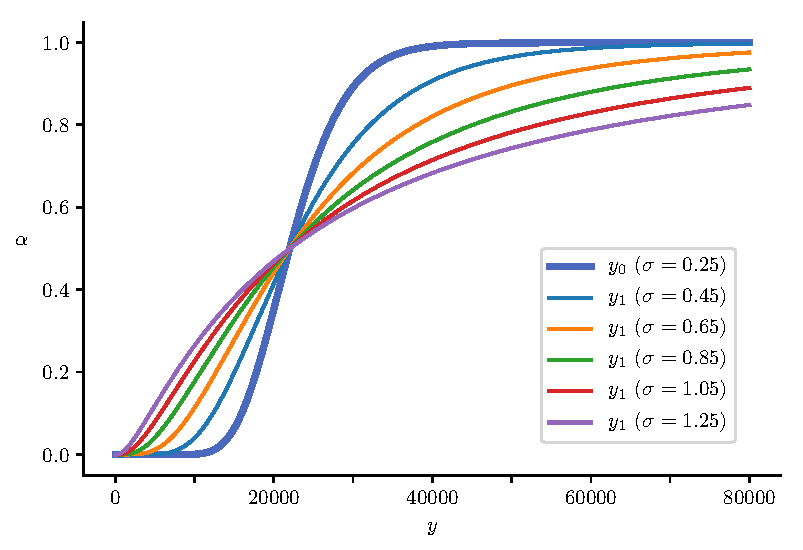
\includegraphics[width = 0.6\textwidth]{RAjointDistribs}
		\vspace{-1ex}
		\floatfoot{\begin{minipage}{0.7\textwidth}
			The thick line represents the joint distribution at $t = 0$. The thin lines are five different examples of joint distributions at $t = 1$, varying in the value of $\sigma_{1}$.
		\end{minipage}}
	\end{figure}
	
Under these parameters and according to \eqref{eq:alphabar}, the optimal choice of $\overline{\alpha}$ at $t = 0$ is
	\begin{equation} \label{eq:exAlphaBar}
		\overline{\alpha} 
			= \mathbb{E}[\alpha_{0}] + \frac{\mathrm{Cov}(y_{0}, \alpha_{0})}{\mathbb{E}[y_{0}]}
			= 0.57,
	\end{equation}
which is 14\% bigger than the mean of the distribution of $\alpha$.\footnote{\,Since $\alpha \sim U(0,1)$, $E[\alpha] = 0.5$.} Now, suppose that between $t = 0$ and $t = 1$ there is a redistribution of income between each of the two halves of the distribution determined by the median. In particular, I assume there is a ``transfer'' from the poorest to the richest half. A modification like this could occur for example, after an unequal growth in income or after a financial crisis. To generate this change I take $y_{1} \sim \log\text{-Normal}(\mu, \sigma_{1})$, with $\sigma_{1} \geq \sigma_{0}$. To see the effects that different values of $\sigma_{1}$ have in the estimation error I consider $\sigma_{1} \in [0.25, 1.25]$. Note that both $y_{0}$ and $y_{1}$ have the same median but the tails of both distributions are heavier, as shown in \Cref{fig:LogNormalSigma1}.\footnote{\,The median of a $\log$-Normal distribution with parameters $\mu$ and $\sigma$ is $e^{\mu}$. For $\mu = 10$, we have that $e^{\mu} \approx 22\,026$.} I assume that the joint distribution at $t = 1$, $F_{1}$, still satisfies $S_{1} = \{(y,\alpha) : P(y_{0} \leq y) = \alpha\}$ and thus is constructed using the same algorithm. This assumptions means that the redistribution did not change the rank of each individual. In order to illustrate the differences between $S_{0}$ and the different supports $S_{1}$, in \Cref{fig:JointDistributions} I show both sets, using the same values for $\sigma_{1}$ as in \Cref{fig:LogNormalSigma1}. From \Cref{fig:JointDistributions} it is clear that given that more mass is moved to the tails of the income distribution, preferences grow more quickly at the beginning of the interval $(0, \infty)$ and higher values of $\alpha$ are restricted to high values of $y$.
	\begin{figure}
		\caption{Densities of $y_{0}$ and $y_{1}$ for different values of $\sigma_{1}$}
		\label{fig:LogNormalSigma1}
		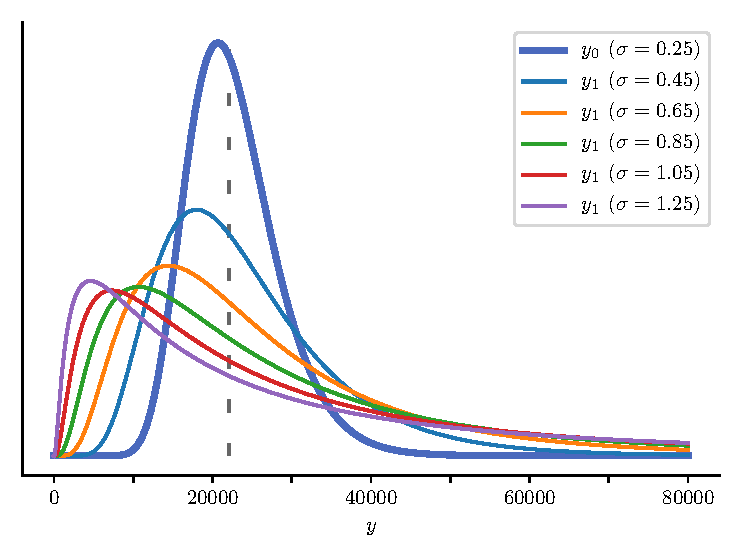
\includegraphics[width = 0.6\textwidth]{RAwageDistribs}
		\floatfoot{\begin{minipage}{0.7\textwidth}
			All distributions have $\mu = 10$ and $\sigma$ according to the legend. The thick line represents the income distribution at $t = 0$. The thin lines are five different examples of distributions at $t = 1$. The dashed gray line corresponds to the common median at, approximately, 22\,026.
		\end{minipage}}
	\end{figure}

It follows from \Cref{fig:JointDistributions} that the covariance between $\alpha$ and $y_{1}$ changes depending on the value of $\sigma_{1}$. Hence, according to \eqref{eq:errorT1} and \eqref{eq:errorT1equalAlpha}, the estimation error changes with $\sigma_{1}$. In \Cref{fig:RADiffPlot} I show the relationship between the estimation error, $D(\overline{\alpha})$ and $\sigma_{1}$ for $0.25 \leq \sigma_{1} \leq 1.25$ in monetary terms. The maximum difference is close to 10\,000 which representes nearly half of the median income.\footnote{\,10\,000 is approximately 0.45 times the median income.} The figure also shows that the error is monotone in $\sigma_{1}$ and weakly convex, as can be seen from the proximity of the curve to the straight line that joins the extremes. Finally, observe that the error is positive for all the considered values of $\sigma_{1}$ and the reason comes directly from the particular construction of this example. Since the covariance between $y_{0}$ and $\alpha$ is always positive and grows (or stalls) at $t=1$, then $M_{1} \geq M_{0}$ for all values of $\sigma_{1}$ (see \eqref{eq:alphabar}) and thus according to \eqref{eq:errorT1}, $D_{1}(\overline{\alpha}) \geq 0$ for every $\sigma_{1}$.
	\begin{figure}
		\caption{Estimation error $D_{1}(\overline{\alpha})$ as a function of $\sigma_{1}$}
		\label{fig:RADiffPlot}
		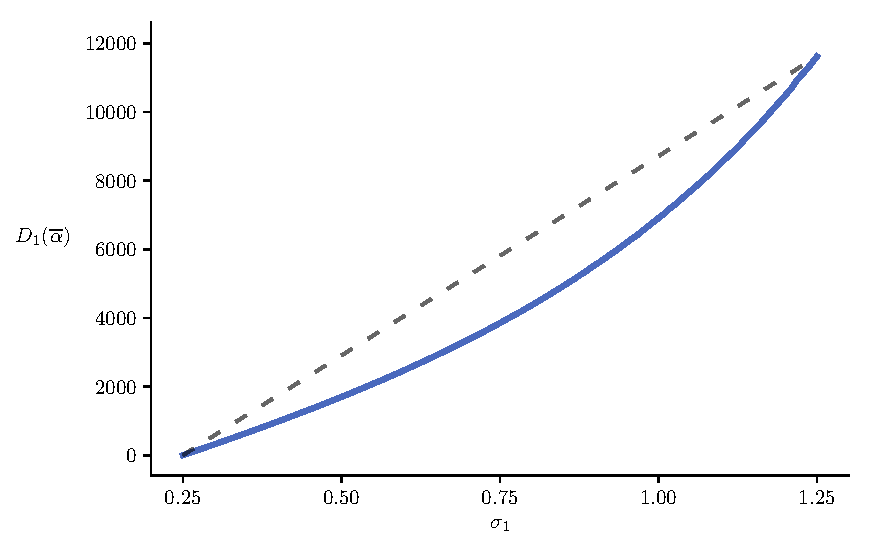
\includegraphics[width = 0.6\textwidth]{RAdiffPlot}
		\floatfoot{\begin{minipage}{0.7\textwidth}
			The blue line shows $D_{1}(\overline{\alpha})$ as a function of $\sigma_{1}$. The dashed gray line joins the two extremes of the curve.
		\end{minipage}}
	\end{figure}
	
\newpage
As noted in \eqref{eq:exAlphaBar}, the value of $\overline{\alpha}$ was slightly over the mean value of the preference marginal distribution. From the previous exercise at least two questions arise:
	\begin{enumerate}
		\item How different is the optimal $\overline{\alpha}$ in \eqref{eq:exAlphaBar} from those needed to reduce the error to zero at $t = 1$?
		\item Is it possible, in the context of this setting, to obtain optimal $\overline{\alpha}$ that completely cover the $(0,1)$ interval?  
	\end{enumerate}
Both questions are closely related, since each one requires studying the response of $\overline{\alpha}$ to changes in the value of $\sigma_{1}$. However, the answers point to different aspects of this setting. The solution to the first question may give additional insights about how sensitive is the model to the choice of parameters. For example, if the relationship between the optimal $\overline{\alpha}$ at $t = 1$ and $\sigma_{1}$ is strongly convex, then a representative agent model is very reactive to even the smallest changes in the underlying heterogeneity of the economy. On the other hand, the answer to the second question illustrates how unrestrained the error can be in the parameter selection even in a simple model like the one presented here. Observe, however, that in this setting, given that $\rmx{Cov}(y_{1},\alpha) \geq 0$, the value of $\overline{\alpha}$ is always greater or equal than $\mathbb{E}[\alpha] = 0.5$ (see \eqref{eq:alphabar}).

To address the first question I compute $M_{1}$ (that according to \eqref{eq:alphabar} is equal to the optimal $\overline{\alpha}$ at $t = 1$) for the different values of $\sigma_{1} \in [0.25, 1.25]$ and plot them in \Cref{fig:RAalphaDiff}. The figure shows that the optimal value of $\overline{\alpha}$ grows fairly linear with $\sigma_{1}$ in this range, which is illustrated by the closeness of both the blue and gray lines. Note that for $\sigma_{1} = 1.25$ the optimal $\overline{\alpha}$ is approximately equal to $0.811$ which is 42.3\% bigger than the chosen value of $0.57$.

	\begin{figure}[h]
		\caption{Optimal $\overline{\alpha}$ at $t = 1$ as a function of $\sigma_{1}$}
		\label{fig:RAalphaDiff}
		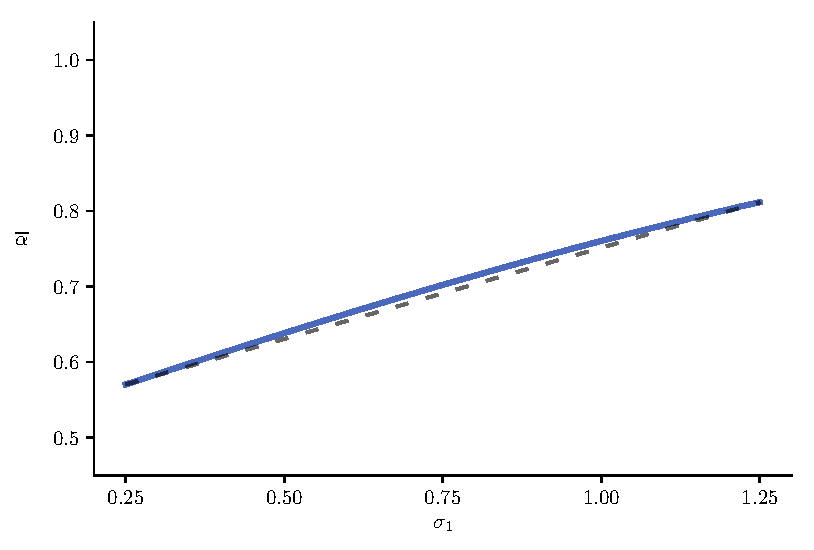
\includegraphics[width = 0.6\textwidth]{RAdiffAlphasPlot}
		\vspace{-1ex}
		\floatfoot{\begin{minipage}{0.7\textwidth}
			The blue line shows the optimal $\overline{\alpha}$ at $t = 1$ as a function of $\sigma_{1}$. The dashed gray line joins the two extremes of the curve. Note that for $\sigma_{1} = 0$, the optimal value of $\overline{\alpha}$ is the same as the one computed at $t = 0$, approximately at $0.57$ (see \eqref{eq:exAlphaBar}).
		\end{minipage}}
	\end{figure}
	
Now, to find an answer to the second question, I conduct the following exercise. I take the same distributions as before, that is, $\alpha \sim U(0,1)$, $y \sim \log\text{-Normal}(\mu, \sigma)$ with $\mu = 10$ and allow $\sigma$ to move between 0 and 5. As before, the joint distribution of $(y,\alpha)$ satisfies the same condition over its support. Next, I compute the optimal $\overline{\alpha}$ using \eqref{eq:alphabar} for these parameters and plot them in \Cref{fig:RAoptimalAlphas}. As mentioned above, $\overline{\alpha} \geq 0.5$ for every $\sigma$ in the considered range. Observe that the curve is highly concave, meaning that $\overline{\alpha}$ can be highly sensitive to the change of $\sigma$. In fact, the growth in the optimal $\overline{\alpha}$ is very steep at the beginning, reaching $0.9$ approximately at $\sigma = 1.83$.\footnote{\,For $\sigma = 1.809$, $\overline{\alpha} = 0.899$ and for $\sigma = 1.834$, $\overline{\alpha} = 0.902$.} Additionally, growth after $\sigma = 2.91$ is greatly reduced: The derivative at this point is 0.01 and since $\overline{\alpha} = 0.98$, then the semi-elasticiy is also close to 0.01.\footnote{The semi-elasticity of $\overline{\alpha}$ in this context is $\frac{1}{\overline{\alpha}} \cdot \pfpx{\overline{\alpha}}{\sigma}$} The previous calculation implies that from 0.98 onwards the growth in $\overline{\alpha}$ is lower than 1\%.  It is also interesting to highlight the opposite curvature of the functions in \Cref{fig:RADiffPlot,fig:RAoptimalAlphas}. According to \eqref{eq:alphabar} and \eqref{eq:errorT1}, the error is a multiple of the difference between the optimal $\overline{\alpha}$ and thus what drives the convexity of the curve in \Cref{fig:RADiffPlot} must be the growth in the mean of $y_{1}$. As a final remark, note that, although this setting does not allow $\overline{\alpha} < 0.5$, reversing the covariance between $\alpha$ and $y$ produces a similar picture as that of \Cref{fig:RAoptimalAlphas}, but the curve is concave decreasing instead of increasing and with an asymptote at $\overline{\alpha} = 0$.

	\begin{figure}[tbh!]
		\caption{Optimal $\overline{\alpha}$ at $t = 1$ as a function of $\sigma$}
		\label{fig:RAoptimalAlphas}
		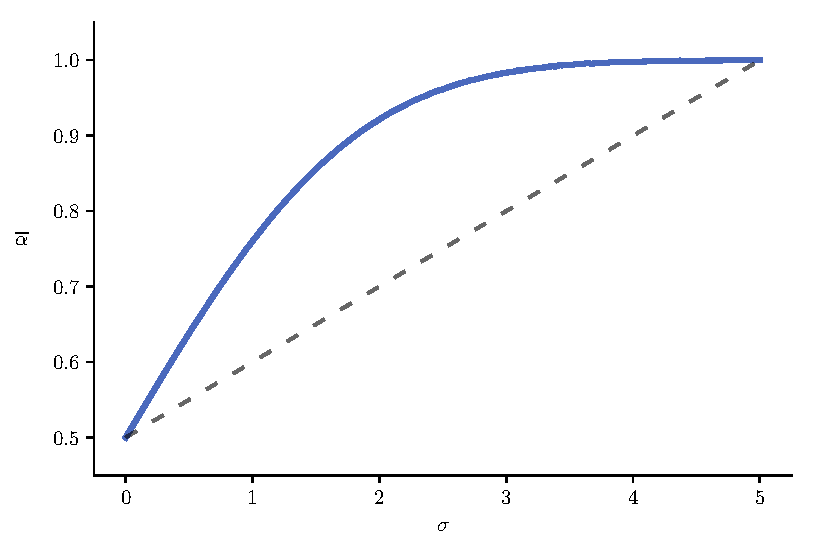
\includegraphics[width = 0.6\textwidth]{RAoptimalAlphas}
		\vspace{-1ex}
		\floatfoot{\begin{minipage}{0.7\textwidth}
			The blue line shows the optimal $\overline{\alpha}$ as a function of $\sigma$, computed according to \eqref{eq:alphabar}, with $\alpha \sim U(0,1)$ and $y \sim \log\text{-Normal}(\mu, \sigma)$, with $\mu = 10$. The dashed gray line joins the two extremes of the curve.
		\end{minipage}}
	\end{figure}

%%%	Consumer aggregation in dynamic models	%%%
\section{Consumer aggregation in dynamic models} \label{sec:CarrollAgg}

	%%	The model	%%
\subsection{The model}
Consider the following model where a consumer, identified with parameters $(\rho, \beta)$ solves the following problem
	\begin{equation} \label{eq:CarrollModel}
		\probop[s.t.]{\max_{\{c_{t}\}_{t}}}{\sum_{t=1}^{\infty} \beta^{t}\frac{c_{t}^{1-\rho}}{1-\rho}}
					{&	k_{t+1} = (1-\delta)(y_{t} - c_{t+1})	\\
					&	y_{t} = k_{t} + \theta_{t}k_{t}^{\alpha}},
%		\probop[s.t.]{\max}{\mathbb{E}_{0}\left[\sum_{t=0}^{\infty} \beta^{t} \frac{C_{t}^{1-\rho}}{1-\rho} \right],}
%				{&	K_{t+1} = (1-\delta)(Y_{t} - C_{t}),	\\
%				&	Y_{t+1} = K_{t+1} + \theta_{t+1}K_{t+1}^{\alpha}L_{t+1}^{1-\alpha},}
	\end{equation}
where $C_{t}$ is consumption at time $t$, $K_{t+1}$ is the capital at the start of period $t+1$ and $Y_{t}$ represents the total resources available (income) at time $t$. Let $c(y)$ represent the infinite-horizon consumption as a function of current resources, where both variables are normalized by permanent labor income, that is, $y = \frac{Y}{wL}$ and similarly for $c$.\footnote{\,If $c_{t}(y)$ is the optimal normalized consumption as a function of normalized current resources, then $c(y) := \lim_{n \to \infty} c_{T-n}(y)$, where $T$ is the last period of the finite horizon counterpart of problem \eqref{eq:CarrollModel}.} A salient feature of these models is that $c$ is a highly concave function of $y$, but for low and high values of income the function is nearly linear, as in \Cref{fig:concaveC}. This behavior may harm predictions of the (aggregate) marginal propensity of consumption (MPC) using a representative agent model if the aggregate income is high but wealth is very unequally distributed. As expected, the difference between empirically estimated MPCs and the one predicted by the representative agent model is substantial, while the former are found between 0.2 and 0.5, the latter is only 0.04 under standard parameters.\footnote{\,See \cite{CarrollRequiem}.}
	\begin{figure}[H]
		\caption{Consumption function}
		\label{fig:concaveC}
		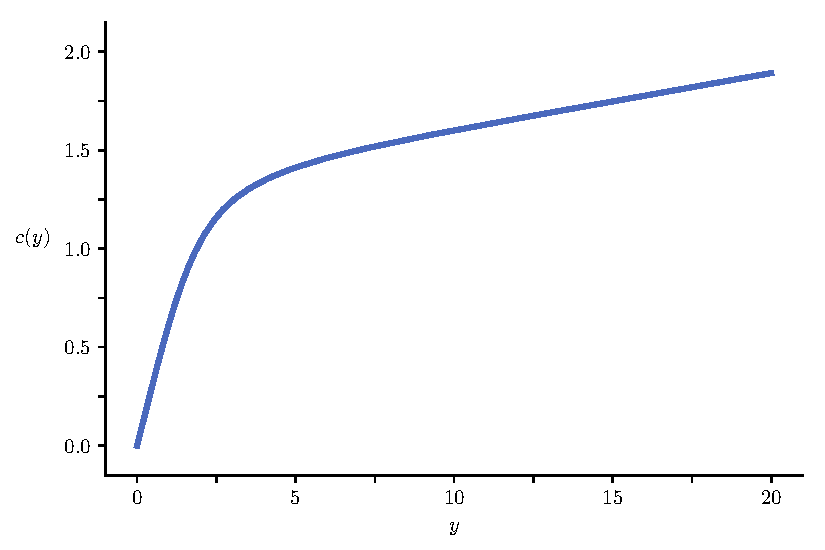
\includegraphics[width=0.6\textwidth]{CarrollCons}
		\vspace{-1ex}
		\floatfoot{\begin{minipage}{0.7\textwidth}
			The blue line shows the (normalized) consumption as a function of the cash-on-hand $y$. The model that produces this type of function includes permanent and idiosyncratic shocks, as in \cite{KrusellSmith98}.
		\end{minipage}
}
	\end{figure}
	
One way to make better predictions is to modify the model to produce a skewed distribution of income, more similar to the data. Of course, if that same data hints how to choose the parameters of the representative agent model, then its use can produce more reasonable estimates without incorporating more complexity. Hereinafter I use the same argument as the one in \Cref{sec:RepAg} to understand how the basic representative agent model in \eqref{eq:CarrollModel} can be calibrated to obtain a better prediction for the MPC.

	%%	The problem of estimating the MPC	%%
\subsection{The problem of estimating the MPC}
Suppose the economy is composed by agents identified by their preference parameters ($\beta$, $\rho$) and their income $y$, distributed according to $F$ with marginals $F_{\beta, \rho}$ and $F_{y}$, respectively. According to the model in \eqref{eq:CarrollModel}, for every pair $(\beta,\rho)$ there is an optimal consumption $c_{\beta,\rho}$ and thus the (aggregate) MPC is 
	$$ \mathrm{MPC}(F) = \int_{S} c_{\beta,\rho}'(y) \, dF, $$
where $S := \supp F$ is the support of the distribution $F$. Note that using the law of total expectation we can write
	\begin{equation} \label{eq:lteMPC}
		\mathrm{MPC}(F) = \mathbb{E}_{y}\Big[ \mathbb{E}_{(\beta,\rho) \, | \, y}[c'_{\beta,\rho}(y)] \; \Big| \; y \Big].
	\end{equation}
Note that if patience ($\beta$) and risk aversion ($\rho$) are known from income, then \eqref{eq:lteMPC} gives a reasonable method to compute the MPC.

Suppose now that an investigator wishes to compute the MPC for this economy but instead of using an heterogeneous model (because data on preferences may not be available), she chooses a pair of parameters ($\overline{\beta}, \overline{\rho}$) to propose a representative consumer model. Solving \eqref{eq:CarrollModel} for these values gives a consumption function $c_{\overline{\beta}, \overline{\rho}}$. Suppose this researcher has access to $F_{y}$, that is, she has data on income. As discussed in \Cref{sec:RepAg}, the previous modeling decision is equivalent to approximating $F_{\beta,\rho}$ by a Dirac distribution $\delta_{\overline{\beta},\overline{\rho}}$ or, in more broader terms, approximate $F$ by another distribution $G$ with marginals $\delta_{\overline{\beta},\overline{\rho}}$ and $F_{y}$ and with the same support. Hence, the MPC in this context is
	\begin{equation} \label{eq:aggMPC}
		\mathrm{MPC}(G) 
			= \int_{S} c_{\overline{\beta},\overline{\rho}}'(y) \, dG 
			= \mathbb{E}_{y}\Big[ c_{\overline{\beta},\overline{\rho}}'(y) \Big].
	\end{equation}	
Thus, using \eqref{eq:lteMPC} and \eqref{eq:aggMPC}, the estimation error with sign is
	$$D(\overline{\beta}, \overline{\rho})
		:=	\mathbb{E}_{y}\Big[ \mathbb{E}_{(\beta,\rho) \, | \, y}[c'_{\beta,\rho}(y) -  c_{\overline{\beta},\overline{\rho}}'(y) ] \; \Big| \; y \Big].$$
This means that, as shown in \Cref{sec:RepAg}, the estimation error arises from differences in the ``estimated'' MPC for each agent. Of course, the aggregate model is not in principle capturing directly the individual MPC. Nevertheless when thought of it as approximating the heterogeneity in the economy, then it is possible to interpret that is indeed the case.

Sadly, for a model like \eqref{eq:CarrollModel} there is no analytic expression for $c_{\beta,\rho}$ and thus neither one for $c'_{\beta,\rho}$. Still, conditional on having a Taylor approximation to a given desired degree of precision, it is clear that these functions depend on a finite amount of moments of the joint distribution of $\beta$, $\rho$ and $y$. Hence, $D(\overline{\beta}, \overline{\rho})$ also depends on a finite number of moments of $F$, allowing a tailoring in the approximation of the heterogeneity with the objective of reducing the estimation error.

	%%	Numerical example	%%
\subsection{Numerical example}
In this section I show that an optimally chosen representative agent model can provide close estimates of the aggregate MPC without modeling the heterogeneity of the population. As mentioned above, every pair $(\beta,\rho)$ in the economy is associated with a consumption function $c_{\beta,\rho}$ from which the MPC at the respective income value $y$ is obtained. To assess how different the policy functions are depending on these parameters, observe \Cref{fig:ConsRhoBeta}. 

	\begin{figure}[H]
		\caption{Consumption functions at different values of $\rho$ and $\beta$} \label{fig:ConsRhoBeta}
		
		\subfloat[$\beta = 0.99$]{\includegraphics[width = 0.45\textwidth]{CarrollConsRho} \label{fig:ConsRho}}\hspace{0.02\textwidth}
		\subfloat[$\rho = 3$]{\includegraphics[width = 0.45\textwidth]{CarrollConsBeta} \label{fig:ConsBeta}}
		\vspace{-1ex}
		\floatfoot{\begin{minipage}{0.95\textwidth}
			Each line is a different consumption function. In Panel (a), $\beta = 0.99$ for all values of $\rho$. Similarly, in Panel (b) for all different consumption functions, $\rho = 3$.
		\end{minipage}}
	\end{figure}

In Panel (a), where $\beta$ is fixed at 0.99 and $\rho$ varies from 1 to 5, the concavity of the function is greater as $\rho$ grows. It is also interesting to note that the curves are almost parallel for high-income agents, meaning that for different values of $\rho$, the MPC is very similar if $y$ is large enough. On the other hand, in Panel (b), $\rho$ is fixed at 3 and $\beta$ varies from $0.89$ to $0.99$. All functions are fairly similar but, again, the concavity increases as $\beta$ gets closer to $0.99$. Contrary to what was shown in Panel (a), the curves have different slopes for large values of $y$, meaning that the MPC differs significantly for each $\beta$. As a final remark, note that the smooth transitions showed in this figure strongly suggest that the choice of the parameters of a representative agent model can balance the underlying heterogeneity of the agents' policy functions when estimating the aggregate MPC.
	
In order to make the last point explicit, consider the following setting. There are $200$ agents in the economy with $\beta$, $\rho$ and $y$ independent random variables. The distribution $F$ is obtained by first taking 200 independent draws from the following distributions:
	\begin{itemize}
		\item $\beta$: triangular distribution with lower limit $0.9$, and with upper limit and mean equal to $0.99$.
		\item $\rho$: triangular distribution with lower limit $1$, upper limit $5$ and mean $3$.
		\item $y$: uniform distribution over the interval $[0,10]$. 
	\end{itemize}

Then, a triple $(\beta,\rho,y)$ is associated to each agent. The distribution of $(\beta,\rho)$ in the economy is presented in \Cref{fig:distribBetaRho}. As can be seen in the figure, the majority of agents are close to the intersection of the dashed lines, that correspond to the mean (and mode) of the underlying distributions. The joint distribution of the triples $(\beta,\rho,y)$ is presented in \Cref{fig:JointDistrib} to further illustrate the independency of the variables.
	\begin{figure}[H]
		\caption{Distribution of $\beta$ and $\rho$ in the economy}
		\label{fig:distribBetaRho}
		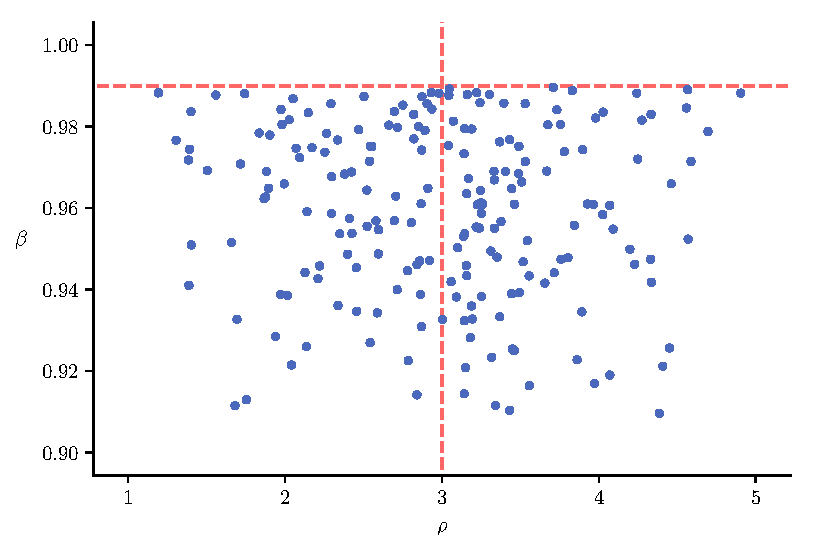
\includegraphics[width=0.6\textwidth]{CarrollDistrib}
		\floatfoot{\begin{minipage}{0.7\textwidth}
			The figure shows the marginal distribution $F_{\beta,\rho}$. Each dot represents an agent in the economy. The dashed lines correspond to $\rho = 3$ and $\beta = 0.99$, the means of the triangular distributions.
		\end{minipage}}
	\end{figure}

	
	\begin{figure}[H]
		\caption{Joint distribution of $\beta$, $\rho$ and $y$ in the economy}
		\label{fig:JointDistrib}
		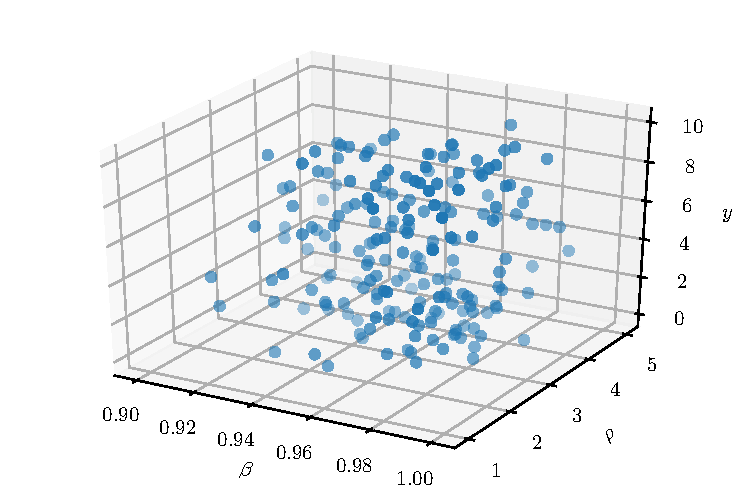
\includegraphics[width=0.6\textwidth]{CarrollDistrib3d}
		\floatfoot{\begin{minipage}{0.7\textwidth}
			The figure shows the distribution $F_{\beta,\rho,y}$. Each dot represents an agent in the economy.
		\end{minipage}}
	\end{figure}

According to the previous section, the joint distribution generated this way determines an aggregated MPC and the choice of $(\overline{\beta}, \overline{\rho})$ is aimed to keep $D(\overline{\beta}, \overline{\rho})$ close to zero. Assuming the only known feature of the distribution of $(\beta, \rho)$ is its boundaries -- in this example, $\beta \in [0.9, 0.99]$ and $\rho \in [1,5]$ -- then I construct a grid with $10\,000$ points by taking 100 evenly spaced points from each interval and making all possible combinations. Next, for each pair $(\overline{\beta}, \overline{\rho})$ I compute the $MPC$ associated to a representative agent model with these parameters. The MPCs computed using this procedure are showed in \Cref{fig:MPCPlane}. 
	\begin{figure}[H]
		\caption{Computed MPC for each pair $(\overline{\beta}, \overline{\rho})$}
		\label{fig:MPCPlane}
		\includegraphics[width=0.6\textwidth]{CarrollMPC}
		\floatfoot{\begin{minipage}{0.7\textwidth}
			The figure shows the computed MPC for each pair $\left(\overline{\beta}, \overline{\rho}\right)$ in a 10\,000 point grid constructed in $[0.9, 1] \times [1,5]$. The red plane is set at the real value of the MPC for this economy, approximately at 0.176. 
		\end{minipage}}
	\end{figure}

\newpage
From the figure it is clear that the blue and red planes intersect in more than one point. Moreover, the intersection is a curve. The figure also shows that the estimated MPC is more responsive to $\beta$ than to $\rho$, which is clear from the higher slope that the blue surface has on the $\overline{\beta}$ axis relative to the $\overline{\rho}$ one. The previous observation is in line with \cite{CarrollRequiem}, where the choice of two different $\beta$ values is crucial to obtain a closer estimate of the MPC. 

%The difference $D(\overline{\beta}, \overline{\rho})$ is also presented in \Cref{fig:DiffPlane}. Again is clear than the difference can get as close as zero as desired and, moreover, that the choice of parameters is not unique.
%
%	\begin{figure}[H]
%		\caption{Difference between real and estimated MPCs for each pair $\left(\overline{\beta}, \overline{\rho}\right)$}
%		\label{fig:DiffPlane}
%		\includegraphics[width=0.6\textwidth]{CarrollDiff}
%%		\floatfoot{\begin{minipage}{0.7\textwidth}
%%			The figure shows $D(\overline{\beta}, \overline{\rho})$ for each pair of the grid.
%%		\end{minipage}}
%	\end{figure}
	
Finally, to give an idea of how the mentioned curve looks, in \Cref{fig:ZeroCurve} I graph the ``zero'' difference curves, that is, the points $(\overline{\beta}, \overline{\rho})$ for which $|D(\overline{\beta}, \overline{\rho})|$ is less than or equal than a certain tolerance. In Panel (a) the tolerance is set to $10^{-4}$ while in Panel (b) it is set to $10^{-5}$. As seen in this figure, the curve is fairly smooth and again shows that the difference is more sensitive to the choice of $\overline{\beta}$ than that of $\overline{\rho}$. This can be seen in the fact that when the tolerance is $10^{-4}$, for every value of $\overline{\rho}$ there is a $\overline{\beta}$ such that the difference is below the tolerance level but the converse is not true. This observation brings back the discussion over \Cref{fig:ConsRhoBeta}. The reason why choosing $\overline{\beta}$ is more critical than choosing $\overline{\rho}$ can be derived following two steps. First, the MPC for different values of $\rho$ is fairly similar for $y > 2$, as evidenced by the similarity of the slopes in Panel (a) of \Cref{fig:ConsRhoBeta}. Second, the 80\% of the uniform distribution over $[0,10]$ is contained in the interval $[2,10]$. Hence, the majority of the agents lie in a portion of the income distribution where the difference in $\rho$ is not significant in the calculation of the MPC. On the contrary, since the MPC for different values of $\beta$ may differ greatly, then the range of optimal $\overline{\beta}$ available could be greatly reduced if tolerance is small enough. In the same line, note that decreasing the tolerance by one order of magnitude strongly reduces the set of optimal parameters available.
	\begin{figure}[H]
		\caption{``Zero'' difference curves}
		\label{fig:ZeroCurve}
		
		\subfloat[tolerance = $10^{-4}$]{\includegraphics[width=0.45\textwidth]{CarrollMPCCurve_-4}}\hspace{0.02\textwidth}
		\subfloat[tolerance = $10^{-5}$]{\includegraphics[width=0.45\textwidth]{CarrollMPCCurve_-5}} 
		
		\vspace{-2ex}
		\floatfoot{\begin{minipage}{0.95\textwidth}
			The figure shows pairs $(\overline{\beta}, \overline{\rho})$ for which $|D(\overline{\beta}, \overline{\rho})|$ is less or equal than a certain tolerance.
		\end{minipage}}
	\end{figure}

%%%	Consumer aggregation and category goods	%%%
\section{Consumer aggregation and category goods} \label{sec:MixedAgg}

	%%	Description	%%
\subsection{Description}
Consider a two period economy composed by agents that consume $n+1$ goods: an essential good $z$ (e.g., water) and $n$ different goods grouped in the vector $\mathbf{x}$. Good $z$ is valued at price $q \in \mathbb{R}_{++}$ and the $\mathbf{x}$ goods are valued at prices $\mathbf{p} \in \mathbb{R}^{n}_{++}$.  In what follows and for simplicity of notation, the subscripts $t$ for all variables are omitted unless needed. Each individual in this setting is identified with a pair $(y,\alpha)$, where $y \in (0,\infty)$ is her income and $\alpha \in (0,1)$ determines the form of her pseudo-Cobb-Douglas (PCD) utility function
	$$u_{\alpha}(\mathbf{x},z) := u_{(y,\alpha)}(\mathbf{x},z) = \sum_{j=1}^{n} x_{j}^{\alpha}z^{1-\alpha} = \left(\sum_{j=1}^{n} x_{j}^{\alpha}\right)z^{1-\alpha}.\footnote{\,The choice of this particular utility function is based on the work of \cite{Helpman08}, where they use a similar function to study international trade. The price index in \eqref{eq:priceindex} is also obtained from this work.}$$

Consumers choose how much of the $\mathbf{x}$ goods to consume in each period according to
	\begin{equation} \label{eq:probdisagg}
		\probop[s.t.]{\mathbf{x}(\mathbf{p}, q, y, \alpha) 
			:= \argmax_{\mathbf{x}, z}}{u_{\alpha}(\mathbf{x}, z),}
				{&	\mathbf{p} \mathbf{x} + qz = y.}
	\end{equation} 

The pairs $(y,\alpha)$ follow a distribution $F$ (with marginal distributions $F_{y}$ and $F_{\alpha}$) over their support $S \subset (0,\infty) \times  (0,1)$. In this setting, it is possible to aggregate consumption of the $\mathbf{x}$ goods into a single good $X$ (see \Cref{ssec:HicksAgg}) given by 
	\begin{equation} \label{eq:qtyindex}
		g_{\alpha}(\mathbf{x}) = \left(\sum_{j=1}^{n} x_{j}^{\alpha}\right)^{1/\alpha}.
	\end{equation}
In that case, we have
	\begin{equation} \label{eq:utilagg}
		U(g_{\alpha}(\mathbf{x}), z) := g_{\alpha}(\mathbf{x})^{\alpha}z^{1-\alpha},
	\end{equation}
which is the usual Cobb-Douglas utility function. Hence, by defining $\epsilon := (1-\alpha)^{-1}$ and
	\begin{equation} \label{eq:priceindex}
		P_{\alpha}(\mathbf{p}) :=  \left( \sum_{j=1}^{n} p_{j}^{1-\epsilon} \right)^{\frac{1}{1-\epsilon}},
	\end{equation}
we have that the category demand
	\begin{equation} \label{eq:probagg}
		\probop[s.t.]{X(\mathbf{p}, q, y, \alpha) := \argmax_{X, z}}{U(X,z),}
										{&	P_{\alpha}(\mathbf{p})X + qz = y,}
	\end{equation}
is equal to 
	\begin{equation} \label{eq:Xformula}
		X(\mathbf{p}, q,y,\alpha) = y\,T_{t}(\alpha, \mathbf{p}) := y \frac{\alpha}{P_{\alpha}(\mathbf{p})},
	\end{equation}
and satisfies 
	\begin{equation} \label{eq:aggequality}
		X(\mathbf{p}, q, y, \alpha) = g_{\alpha}\big(\mathbf{x}(\mathbf{p}, q, y, \alpha)\big).
	\end{equation}
This means that the disaggregate model is coherent with the aggregate one for each individual consumer. In other words, aggregation is an exact fit for each agent. Indeed, observe that the price and quantity indices are specific for each agent as they depend on $\alpha$. This means that any attempt to describe this economy using category demands instead of the disaggregate consumption needs knowledge about the heterogeneity of the population in order to avoid approximation errors. Hence, although an exact representation for each consumer is available, doing the same for the economy as a whole requires knowledge about the different preferences, something that is possibly not available to the modeler.

	%%	The prediction problem	%%
\subsection{The prediction problem}
Consider now the following situation. An investigator at time $t = 0$ has data available on disaggregate consumption of the $\mathbf{x}$ and $z$ goods, income (i.e., she knows $F_{y_{0}}$) and prices. Her objective is to estimate the aggregate category demand at $t=1$ (e.g., the country demand for meat next year), $\mathbf{X}_{1}$. For simplicity she assumes that all agents have the same preferences, which means that all differences in consumption are accounted by differences in income. The last assumption also implies that she must choose a single parameter $\overline{\alpha}$ in order to obtain the category demand and the price index of each agent. Again, in the distribution-approximation sense, observe that the mentioned assumption has the same effect I discuss above: The aggregate model imposes an additional level of approximation by replacing  $F_{\alpha}$ with $\delta_{\overline{\alpha}}$. However, note that in this case bundling goods into a category also represents an approximation but of a different nature. Both, $F$ and the function $\mathbf{x}(\mathbf{p}, q, y, \alpha)$ induce a distribution $G$ over the vector $\mathbf{x}$. Then, $g_{\alpha}$ induces a distribution over $X$ that is in some sense an approximation of $G$, due to \eqref{eq:aggequality}. Hence, while the approximation is made directly over $F$, its implications reach $G$ through $g_{\alpha}$.

Under the previous assumption, the best estimation for the category demand of each agent at time $t$ is
	$$\widehat{X}_{t}(\mathbf{p}_{t}, y_{t}, \overline{\alpha}) = y_{t}\, T_{t}(\overline{\alpha}, \mathbf{p}_{t}) = \frac{\overline{\alpha}}{P_{\overline{\alpha}}(\mathbf{p}_{t})}.$$
Thus, the best estimation for the aggregate category demand is
	\begin{equation} \label{eq:AggCatDemand}
		\widehat{\mathbf{X}}_{t}(\mathbf{p}_{t}, F_{y_{t}}, \overline{\alpha}) 
			= \int_{0}^{\infty}y_{t}\, T_{t}(\overline{\alpha}, \mathbf{p}_{t}) \, dF_{y_{t}}
			= \mathbb{E}[y_{t}]\, T_{t}(\overline{\alpha}, \mathbf{p}_{t}).
	\end{equation}

	%%	 A complex estimation error	%%
\subsection{A complex estimation error} \label{ssec:Category-Error}
To understand how the estimation errors appear in this setting I proceed in two steps. First, since category demands depend on $\alpha_{t}$, then for agent $(y_{t},\alpha_{t})$ the true value differs from the estimated one by
	\begin{equation} \label{eq:DtCategory}
		\mathcal{D}_{t}(y_{t},\alpha_{t},\overline{\alpha})
			:=	X(\mathbf{p}_{t}, y_{t}, \alpha_{t}) - \widehat{X}_{t}(\mathbf{p}_{t}, y_{t}, \overline{\alpha})
			=	y_{t}\Big(T_{t}(\alpha_{t}, \mathbf{p}_{t}) - T_{t}(\overline{\alpha}, \mathbf{p}_{t}) \Big).\footnote{\,Note that in this setting $X$ does not depend on $q$ and thus, to simplify notation, this variable was suppressed.}
	\end{equation}

It is not obvious that this difference is monotone in $\overline{\alpha}$ for a given pair $(y_{t}, \alpha_{t})$. In fact, it is not. To see this I take $n = 2$, $\mathbf{p}_{t} = (1,10)$ and present differences $\mathcal{D}_{t}$ relative to income (i.e., as a percentage) as a function of $\overline{\alpha}$ for different values of $\alpha_{t}$ in \Cref{fig:monotDt}.\footnote{\,Choosing this price vector has only clarifying purposes. All of the features mentioned in the rest of the paragraph are maintained if $\mathbf{p}_{t}$ is changed.} For illustrative purposes I restrict $\overline{\alpha}$ to the interval $[0.15, 0.85]$. 
	\begin{figure}[H]
		\caption{$D_{t}$ relative to income as a function of $\overline{\alpha}$}
		\label{fig:monotDt}
		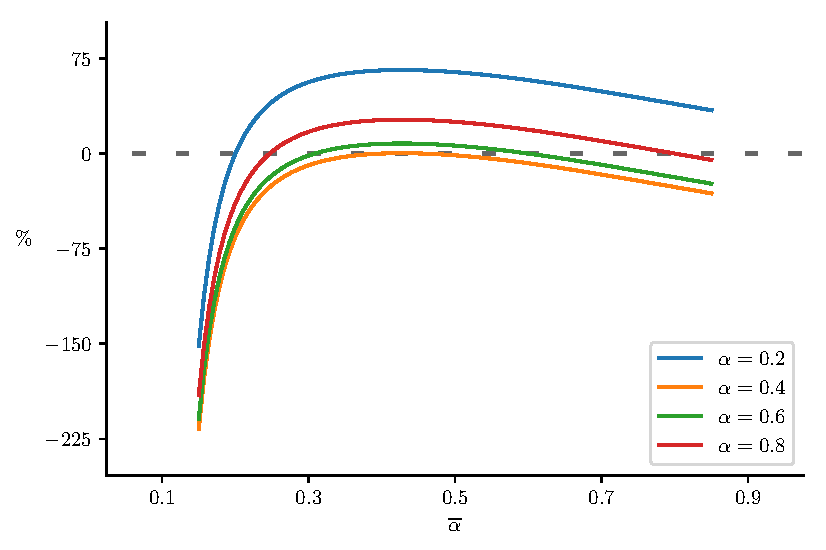
\includegraphics[width = 0.6\textwidth]{MonotonocityDt} \vspace{-1ex}
		\floatfoot{\begin{minipage}{0.7\textwidth} The figure shows $\mathcal{D}_{t}$ relative to income (i.e., $\mathcal{D}_{t}/y_{t} \times 100$) as a function of $\overline{\alpha}$ for the five different $\alpha_{t}$ showed in the legend. The price vector used is $\mathbf{p}_{t} = (1,10)$. The dashed gray line corresponds to $\mathcal{D}_{t} = 0$.
		\end{minipage}}
	\end{figure}

Each curve exhibits a strong non-monotonic behavior and is highly concave, increasing its value quite abruptly when $\overline{\alpha}$ is low and decreasing slowly when $\overline{\alpha}$ is high. Related to the former phenomenon and as showed in the figure, almost all curves cross the horizontal line twice: once when $\overline{\alpha} = \alpha$ in the increasing part of the curve and a second time in a greater value when the relative error is decreasing. The previous characteristic is important when trying to reduce the error to zero because it gives, at first glance, a broader range of optimal $\overline{\alpha}$ to choose. However, it may be the case that the error tolerance is small enough to restrict the attention to higher values of $\overline{\alpha}$ where the relative change in $\mathcal{D}_{t}$ is smaller. The last comment also highlights a curious feature of this setting: An investigator whose objective is reducing the error to zero might be interested in selecting a high value of $\overline{\alpha}$, away from the real values of preferences, in order to protect herself from small changes that could be more harmful when $\overline{\alpha}$ is small. A final insight can be extracted from the transition between the curves. Note that the blue line ($\alpha = 0.2$) moves downward when $\alpha$ grows to 0.4 but all the remaining curves move upward. This behavior relates closely to the one of $T_{t}$, as shown in \Cref{fig:monotTt}, where this variable displays the inverse behavior, decreasing rapidly for small values of $\alpha$ and then growing at a slower rate. 
	\begin{figure}[H]
		\caption{$T_{t}$ as a function of $\alpha$}
		\label{fig:monotTt}
		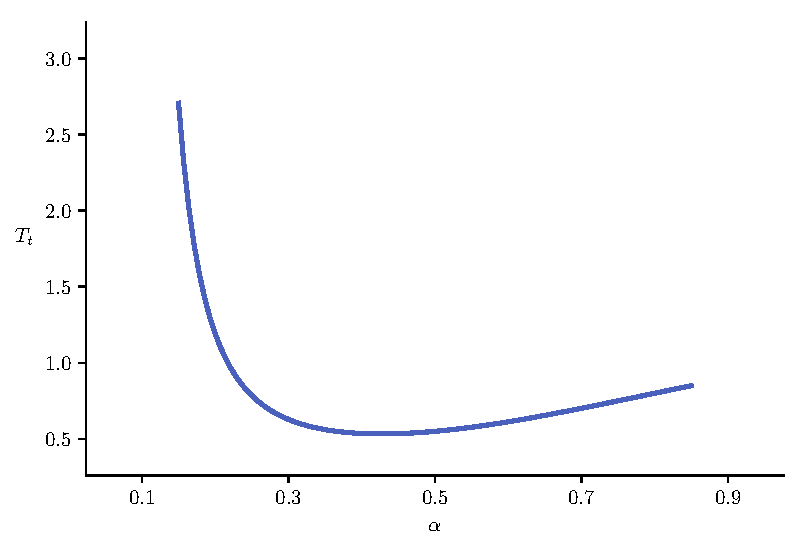
\includegraphics[width = 0.6\textwidth]{MonotonocityTt}
		\vspace{-1ex}
		\floatfoot{\begin{minipage}{0.7\textwidth} The figure shows $T_{t}$ as a function of $\alpha$. The price vector used is $\mathbf{p}_{t} = (1,10)$.
		\end{minipage}}
	\end{figure}

The second step of the analysis consists in studying the aggregate error. To this end, note that the estimation error (with sign) of $\mathbf{X}_{1t}$ is just the integral of $\mathcal{D}_{t}$ over $S$. To simplify notation let $T_{t} = T_{t}(\alpha , \mathbf{p}_{t})$ and $\overline{T}_{t} = T_{t}(\overline{\alpha}, \mathbf{p}_{t})$. In the simplest case where preferences do not change over time we have
	\begin{equation} \label{eq:DiffMix}
	\begin{aligned} 
		D_{t}\left(\overline{T}_{t}\right)
			&:=	\int_{S} \mathcal{D}_{t}(y_{t},\alpha,\overline{\alpha})	\\
			&=	\mathbb{E}\big[y_{t} \, T_{t}\big] - \mathbb{E}[y_{t}]\, \overline{T}_{t}		\\
			&=	\mathrm{Cov}\left(y_{t}, T_{t} \right) + \mathbb{E}[y_{t}]\mathbb{E}\left[T_{t}\right] - \mathbb{E}[y_{t}]\, \overline{T}_{t}	\\
			&= 	\mathbb{E}[y_{t}]\left\{ \frac{\mathrm{Cov}\left(y_{t}, T_{t} \right)}{\mathbb{E}[y_{t}]} + \mathbb{E}\left[T_{t}\right] - \overline{T}_{t} \right\}.
	\end{aligned}
	\end{equation}
which is in principle very similar to \eqref{eq:DiffAgRep} in \Cref{ssec:RepAgError}. However, note now that $D_{t}$ depends on prices and hence on their dynamics. In terms of distributions observe that in this case, the mixed setting implies that the distribution that matters is the one of $(y_{t},T_{t})$ which includes an additional source of heterogeneity: $\mathbf{p}_{t}$. From \eqref{eq:DiffMix} we know that the sufficient statistics needed to obtain an exact fit at time $t$ are, just as in \Cref{ssec:RepAgError}, the first and second moments of that distribution. The difference in this example is that the new source of variation, prices, may affect heavily the precision with which these statistics are estimated.

It is clear from \eqref{eq:DiffMix} that an investigator interested in making the estimation error the smallest possible should choose $\overline{\alpha}$ such that
	\begin{equation} \label{eq:OptT}
		\overline{T}_{t} =  \underbrace{\mathbb{E}\left[T_{t} \right] + \frac{\mathrm{Cov}\left(y_{t}, T_{t} \right)}{\mathbb{E}[y_{t}]}}_{:= \tilde{M}_{t}}.
	\end{equation}

Observe that changes in prices may affect the right hand side of \eqref{eq:OptT}. If the investigator only has access to $t =0$ variables, knowing the price dynamics may not be enough to reduce the estimation error at $t =1$ to zero. Indeed, note that the value of each term in $\tilde{M}_{0}$ is unknown at $t=0$, thus any correction using knowledge about price changes is not feasible. It is interesting to note, however, that if relative prices do not change between $t=0$ and $t=1$, that is, if $\mathbf{p}_{1} = \lambda \mathbf{p}_{0}$, then using that $P_{\alpha}(\mathbf{p})$ is homogeneous of degree 1 we have $T_{1} = \lambda^{-1}T_{0}$,
	$$\lambda^{-1}\tilde{M}_{0} = \mathbb{E}[T_{1}] + \frac{\mathrm{Cov}\left(y_{0}, T_{1} \right)}{\mathbb{E}[y_{0}]},$$
and
	\begin{equation} \label{eq:CorrectT}
		\overline{T}_{1} = \lambda^{-1}\overline{T}_{0}.
	\end{equation}
Hence, in this scenario, setting $\overline{T}_{0} = \tilde{M}_{0}$ as in \eqref{eq:OptT} (assuming that reducing the estimation error to zero at $t=0$ is achievable) and then making the correction in \eqref{eq:CorrectT} further reduces the estimation error if
	\begin{align*}
		\left|\tilde{M}_{1} - \lambda^{-1}\tilde{M}_{0} \right|
			&\leq \left|\tilde{M}_{1} - \tilde{M}_{0} \right|	\\
		\left| \frac{\mathrm{Cov}\left(y_{1}, T_{1} \right)}{\mathbb{E}[y_{1}]} - \frac{\mathrm{Cov}\left(y_{0}, T_{1} \right)}{\mathbb{E}[y_{0}]} \right|
			&\leq \left| \mathbb{E}\left[T_{1} \right] - \mathbb{E}\left[T_{0} \right] + \frac{\mathrm{Cov}\left(y_{1}, T_{1} \right)}{\mathbb{E}[y_{1}]} - \frac{\mathrm{Cov}\left(y_{0}, T_{0} \right)}{\mathbb{E}[y_{0}]} \right|	\\
		\left| \frac{\mathrm{Cov}\left(y_{1}, T_{1} \right)}{\mathbb{E}[y_{1}]} - \frac{\mathrm{Cov}\left(y_{0}, T_{1} \right)}{\mathbb{E}[y_{0}]} \right|
			&\leq \left| (1-\lambda)\mathbb{E}\left[T_{1} \right] + \frac{\mathrm{Cov}\left(y_{1}, T_{1} \right)}{\mathbb{E}[y_{1}]} - \frac{\mathrm{Cov}\left(y_{0}, T_{0} \right)}{\mathbb{E}[y_{0}]} \right|.
	\end{align*}
\newpage \noindent
Moreover, if $y_{1} = Ry_{0}$ for some $R>0$, then implementing this correction eliminates the error, just as what happened in \Cref{ssec:RepAgError}. Finally, note that if prices do not change, then $T_{0} = T_{1}$ and \eqref{eq:DiffMix} has the same form as \eqref{eq:DiffAgRep}. This phenomenon is in line with the previous discussion: By suppressing the variation or heterogeneity in prices over time we return to the results of the model in \Cref{sec:RepAg}.

	%%	Numerical example	%%
\subsection{Numerical example} \label{ssec:Category-Example}
In this section I construct an example in order to understand this particular setting and study how the optimal aggregation parameters and the approximation accuracy change between one period and the next. For this purpose, I take $n = 2$ and $\mathbf{p}_{0} = (1,10)$, I assume preferences do not change (thus, $\alpha_{0} = \alpha_{1} = \alpha$) and consider the same constructions for the joint distributions $F_{0}$ and $F_{1}$ that were presented in \Cref{ssec:RAexample}, except for the fact that, for clarifying purposes, $\alpha$ is restricted to the interval $[0.15, 0.85]$.\footnote{\,This is, $y_{0}$ and $y_{1}$ follow $log$-Normal distributions with parameters $(\mu, \sigma_{0})$ and $(\mu, \sigma_{1})$, respectively, $\alpha \sim U(0.15, 0.85)$ and the joint distribution is such that individuals with higher $\alpha$ have higher income.} In this case I choose $\mu = \ln 5.5$, $\sigma_{0} = 0.25$ and $\sigma_{1} \in [0.25, 1.25]$. This value of $\mu$ ensures that the median consumer can buy half of each of the $\mathbf{x}$ goods. In order to continue the discussion at the end of the previous section I consider $\mathbf{p}_{1} = \lambda\mathbf{p}_{0}$ and two values for $\lambda$, $\lambda_{1} = 0.5$, $\lambda_{2} = 1.5$. This way, with $\lambda_{1}$ the $\mathbf{x}$ goods reduce their cost (relative to $z$) and viceversa with $\lambda_{2}$. The difference between $T_{0}$ and both $T_{1}$ is presented in \Cref{fig:DiffTtLambda}. As can be seen in the image, lower prices rise the value of $T_{1}$ in contrast to $T_{0}$, while greater prices have the opposite effect, as expected from the functional form of $T_{t}$. Since prices appear in the denominator, the increase of $T_{t}$ after a price fall is greater than its drop.\footnote{\,Remember that in this scheme $T_{1} = \lambda^{-1}T_{0}$ and hence, for a given value of $T_{0}$, the function $T_{1}(\lambda)$ behaves like $x^{-1}$.}
	\begin{figure}
		\caption{$T_{0}$ and $T_{1}$ as a function of $\alpha$}
		\label{fig:DiffTtLambda}
		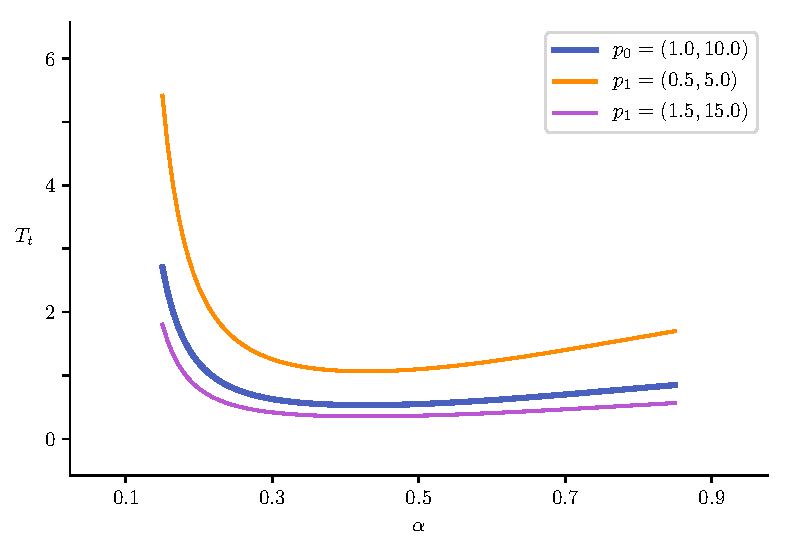
\includegraphics[width = 0.6\textwidth]{TtLambdas}
		\vspace{-1.5ex}
		\floatfoot{\begin{minipage}{0.7\textwidth} The figure shows $T_{0}$ (thick blue line) and $T_{1}$ (yellow and purple lines) as a function of $\alpha$. $T_{0}$ is computed using $\mathbf{p}_{0} = (1,10)$ and each $T_{1}$ is computed with $\mathbf{p}_{1} = \lambda_{i}\mathbf{p}_{0}$, where $\lambda_{1} = 0.5$ and $\lambda_{2} = 1.5$.
		\end{minipage}}
	\end{figure}

In the previous section I mentioned that for this setting the important distribution is the one of $(y_{t}, T_{t})$. Consequently, the next step is to investigate its support in a similar fashion as in \Cref{ssec:RAexample}. In \Cref{fig:JointDistribsCategory} I present the support of the three joint distributions of interest: the one of $(y_{t}, \alpha_{t})$ in \Cref{fig:Jointa}, $(y_{t}, T_{t})$ with $\lambda_{1} = 0.5$ in \Cref{fig:Jointb} and the one of $(y_{t}, T_{t})$ using $\lambda_{2} = 1.5$ in \Cref{fig:Jointc}. It is possible to see that while $y_{t}$ and $\alpha$ have positive covariance, for $y_{t}$ and $T_{t}$ it is negative and in both cases the relation is not monotonic. Additionally, in \Cref{fig:Jointb} we see that this covariance is increased in absolute value between $t = 0$ and $t = 1$, as evidenced by the steeper line that joins the extremes of the $t=1$ curves, which contrasts with the wider line of the $t=0$ variables. The opposite effect is observed in \Cref{fig:Jointc}. It is also worth noting that to the right side of the median, the relation $(y_{t}, T_{t})$ is almost constant in both Panels (b) and (c), while the highest variability happens to income values below the median. Hence, by looking back at \eqref{eq:DtCategory}, it is clear that choosing $\overline{\alpha}$ closer to the one shared by the high-income fraction of the population may reduce the estimation error further than focusing on the complete set of agents. Remembering that using the representative agent means changing the support to a straight horizontal line in each of the panels in \Cref{fig:JointDistribsCategory}, then the previous comment means that in this particular setting, a two-agent model can be a much better approximation, while still maintaining the simplicity. In graphical terms, a two-agent model appears as a two-valued function in each of the plots in \Cref{fig:JointDistribsCategory}.

For this example, the choice of optimal parameters at $t = 0$ is summarized in \Cref{tab:OptimalAlphaT}. The value of $\overline{\alpha}$ is chosen optimally to minimize the (absolute value of the) error at $t = 0$ and then $\overline{T}_{0}$ is computed using the definition. Finally, $\overline{T}_{1}$ is obtained following the aforementioned correction $\overline{T}_{1} = \lambda^{-1}\overline{T}_{0}$. The first two rows of the column are equal precisely because the optimal parameters are obtained at $t =0$, when no price change has yet occurred. The last row is in line with the previous discussion. The optimal $\overline{T}_{1}$ in both cases is closer to the more constant part given by the rich half of the population. The explanation comes directly from \eqref{eq:DtCategory}: Since income is higher for this half, is more important to diminish the difference for these agents than for the other half in order to reduce the error to zero.
	\begin{figure}[H]
		\caption{Support of joint distributions}
		\label{fig:JointDistribsCategory}
		
		\subfloat[$(y_{t},\alpha)$]{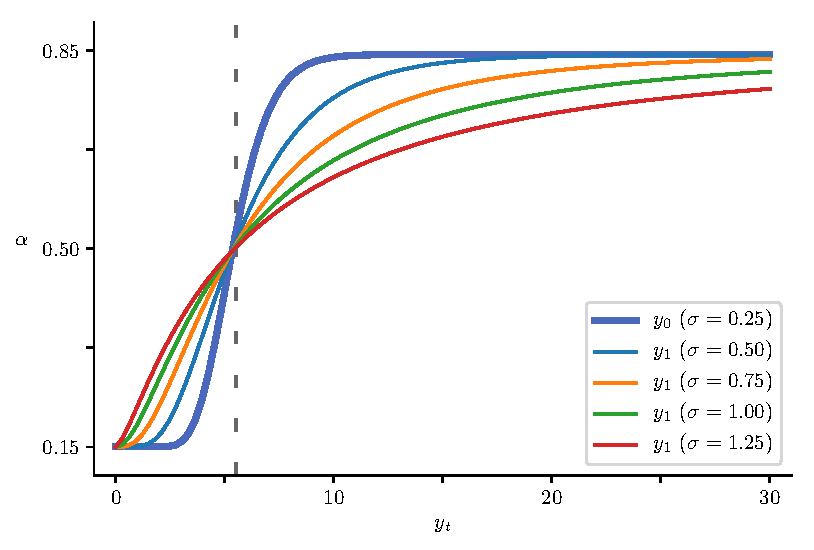
\includegraphics[width = 0.45\textwidth]{JointYA}\label{fig:Jointa}} \vspace{1.5ex}
		
		\subfloat[$(y_{t},T_{t}), \lambda_{1} = 0.5$]{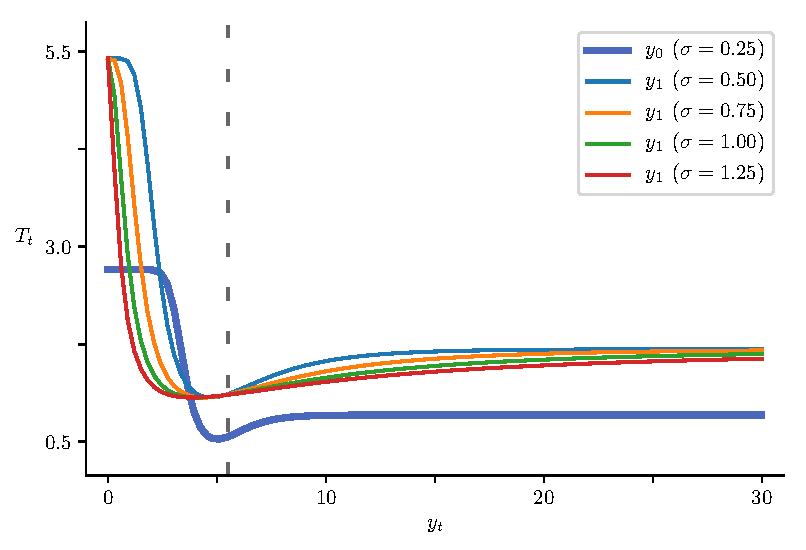
\includegraphics[width = 0.45\textwidth]{JointYT_0}\label{fig:Jointb}}\hspace{0.02\textwidth}
		\subfloat[$(y_{t},T_{t}), \lambda_{2} = 1.5$]{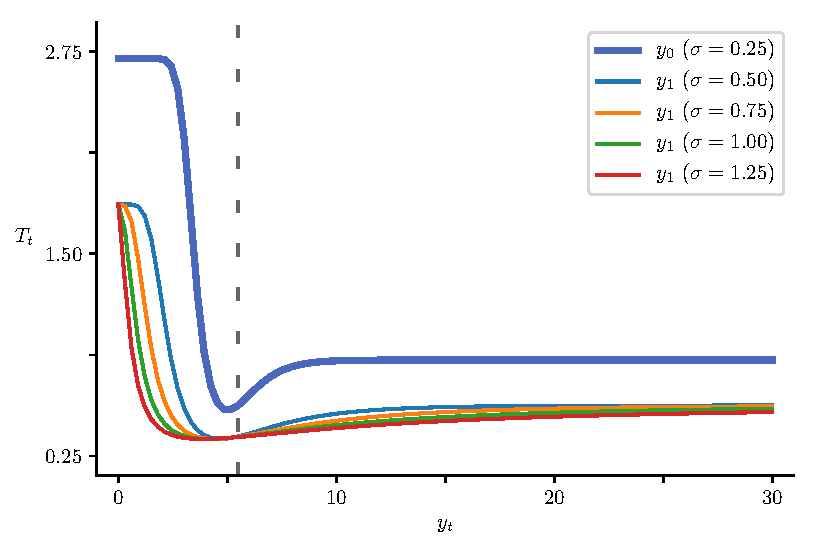
\includegraphics[width = 0.45\textwidth]{JointYT_1}\label{fig:Jointc}}
		
		\vspace{-2ex}
		\floatfoot{\begin{minipage}{0.95\textwidth} The figure shows the support of the joint distributions of $(y_{t}, \alpha)$, $(y_{t}, T_{t})$ with $\lambda_{1} = 0.5$ and $(y_{t}, T_{t})$ with $\lambda_{2} = 1.5$ for five different values of $\sigma_{1}$. The dashed gray lines correspond to $y_{t} = 5.5$, the median of the distribution. The price vectors used are $\mathbf{p}_{0} = (1,10)$ and $\mathbf{p}_{1} = \lambda_{i} \mathbf{p}_{0}$, with $i = 1,2$.
		\end{minipage}}
	\end{figure}

The next step is to determine how big the estimation error is at $t = 1$. \Cref{fig:CategoryDiff1Plot} presents the difference $D_{1}(\overline{T}_{1})$ as a function of $\sigma_{1}$ (see \eqref{eq:DiffMix}), the parameter of redistribution. As we can see from the figure, the approximation error using this corrected parameter is near zero and in both cases the aggregate demand is overestimated. Although meaningless because of the order of magnitude, it is interesting to note that when prices drop, the discrepancy is bigger than when they increase. In other words, when prices fall from $t=0$ to $t = 1$, the overestimation of the aggregate demand is more pronounced. This result should come with no surprise after analyzing \Cref{fig:JointDistribsCategory}. In Panels (b) and (c) we see that the drop in $T_{t}$ after a price increase is smaller than its rise after a price fall. Hence, the change in $X_{1}$ in the first case is smaller than in the second (see \eqref{eq:Xformula}). 
	\begin{table}[H]
		\centering
		\caption{Optimal parameters at $t = 0$}
		\label{tab:OptimalAlphaT}
		\begin{tabular}{ccc}
		\hline\hline
														\\[-2ex]
							&	\multicolumn{2}{c}{$\lambda$}	\\\cline{2-3}
														\\[-2ex]
							&	$0.5$		&	$1.5$	\\ \hline
														\\[-2ex]
			$\overline{\alpha}$	&	$0.75$		&	$0.75$	\\[1ex]
			$\overline{T}_{0}$	&	$0.75$		&	$0.75$	\\[1ex]
			$\overline{T}_{1}$	&	$1.5$		&	$0.5$	\\[.5ex]
		\hline\hline
		\end{tabular} \vspace{2ex}
		
		\begin{minipage}{0.3\textwidth} \scriptsize
			The table shows the optimal parameters $\overline{\alpha}$, $\overline{T}_{0}$ and $\overline{T}_{1} = \lambda^{-1} \overline{T}_{0}$ for the two values of $\lambda$. The price vectors used are $\mathbf{p}_{0} = (1,10)$ and $\mathbf{p}_{1} = \lambda_{i} \mathbf{p}_{0}$, with $i = 1,2$.
		\end{minipage}
	\end{table}

From the discussion at the end of \Cref{ssec:Category-Error}, the correction in \eqref{eq:CorrectT} is useful only if
	$$\left|\tilde{M}_{1} - \lambda^{-1}\tilde{M}_{0} \right|
			\leq \left|\tilde{M}_{1} - \tilde{M}_{0} \right|.$$
Using this numerical example it is possible to determine if the change from $\overline{T}_{0}$ to $\overline{T}_{1}$ is capable of lowering the (absolute value of the) error by directly computing $D_{1}(\overline{T}_{0})$. In \Cref{fig:CategoryDiff0Plot} I show how this difference changes with $\sigma_{1}$. Comparing this figure with \Cref{fig:CategoryDiff1Plot} we see that making the correction lowers the error by several orders of magnitude: While changing the parameter obtained at $t = 0$ using \eqref{eq:CorrectT} gives an error of magnitude $10^{-7}$, keeping $\overline{T}_{0}$ returns an estimate that differs with the real value by $10^{-1}$, six orders of magnitude greater than in the previous case. Nevertheless, it must be borne in mind that in order to use $\overline{T}_{0}$ it is not necessary to know the value of $\lambda$, which may not be available at $t = 0$. If that is the case, the difference found may be small enough to choose to maintain the uncorrected parameter.
	\begin{figure}[H] 
		\caption{Estimation error $D_{1}(\overline{T}_{1})$ as a function of $\sigma_{1}$}
		\label{fig:CategoryDiff1Plot}
		\subfloat[$\lambda = 0.5$]{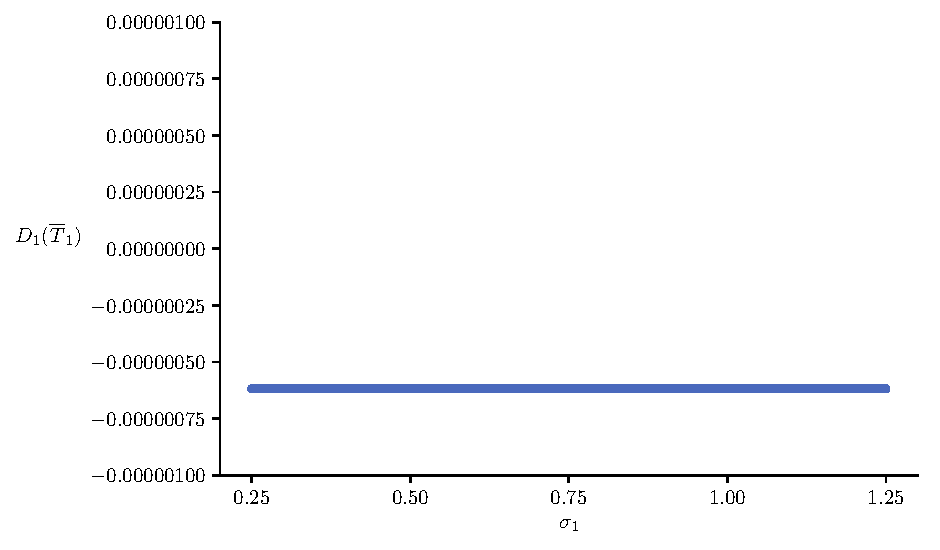
\includegraphics[width = 0.45\textwidth]{Categorydiff1Plot_0} \label{fig:Diffa}}\hspace{0.02\textwidth}
		\subfloat[$\lambda = 1.5$]{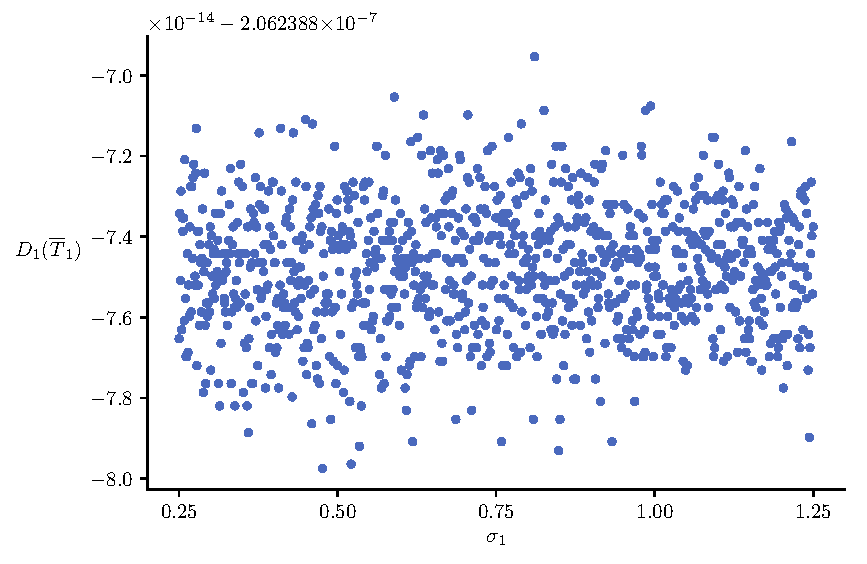
\includegraphics[width = 0.45\textwidth]{Categorydiff1Plot_1} \label{fig:Diffb}}
		
		\vspace{-1.5ex}
		\floatfoot{\begin{minipage}{0.95\textwidth}
			The blue line shows $D_{1}(\overline{T}_{1})$ as a function of $\sigma_{1}$, computed using \eqref{eq:DiffMix}. $\overline{T}_{1}$ is computed using the correction in \eqref{eq:CorrectT}. The price vectors used are $\mathbf{p}_{0} = (1,10)$ and $\mathbf{p}_{1} = \lambda_{i} \mathbf{p}_{0}$, with $i = 1,2$.
		\end{minipage}}
	\end{figure}


	\begin{figure}[H] 
		\caption{Estimation error $D_{1}(\overline{T}_{0})$ as a function of $\sigma_{1}$}
		\label{fig:CategoryDiff0Plot}
		\subfloat[$\lambda = 0.5$]{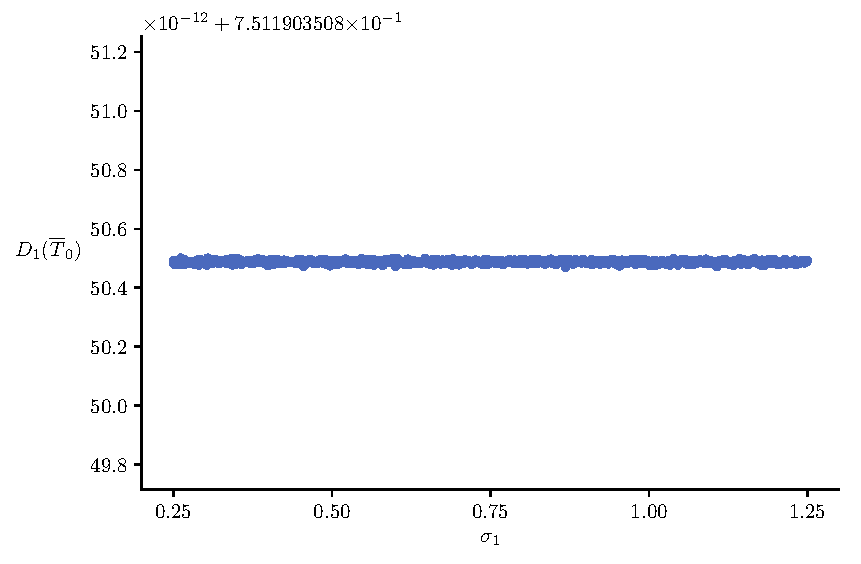
\includegraphics[width = 0.45\textwidth]{Categorydiff0Plot_0} \label{fig:Diffa}}\hspace{0.02\textwidth}
		\subfloat[$\lambda = 1.5$]{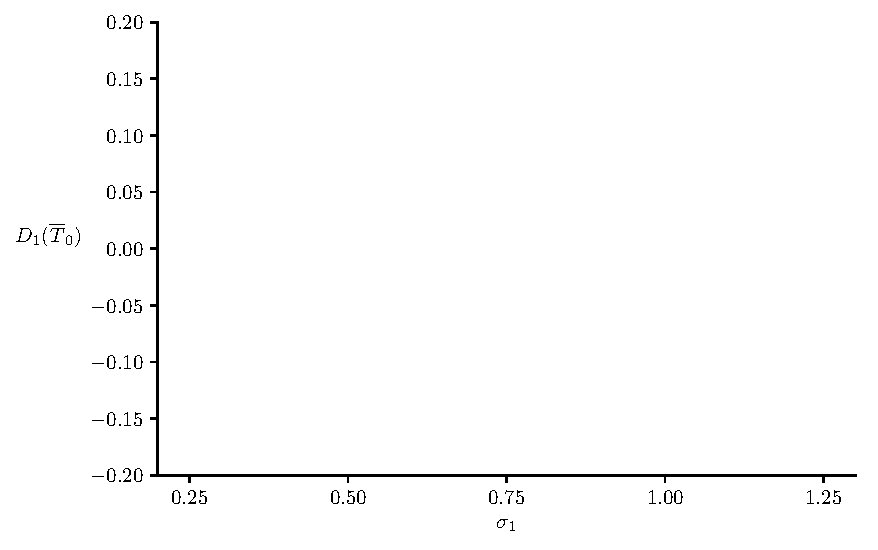
\includegraphics[width = 0.45\textwidth]{Categorydiff0Plot_1} \label{fig:Diffb}}
		
		\vspace{-1.5ex}
		\floatfoot{\begin{minipage}{0.95\textwidth}
			The blue line shows $D_{1}(\overline{T}_{1})$ as a function of $\sigma_{1}$, computed using \eqref{eq:DiffMix}. The price vectors used are $\mathbf{p}_{0} = (1,10)$ and $\mathbf{p}_{1} = \lambda_{i} \mathbf{p}_{0}$, with $i = 1,2$.
		\end{minipage}}
	\end{figure}

To close this section I show how the optimal $\overline{\alpha}$ should evolve depending on the value of $\sigma_{1}$. The results shown in \Cref{fig:CategoryDiff1Plot,fig:CategoryDiff0Plot} suggest that $\overline{\alpha}$ should be constant over time, since the error commited in both cases is small, especially in the first case. In \Cref{fig:CategoryAlphaPlot} I show that this is exactly the case: Both when prices drop and when they increase, the optimal $\overline{\alpha}$ is the same regardless the value of $\sigma_{1}$. The explanation for this phenomenon is, again, obtained directly from \eqref{eq:OptT}. In this example, $\rmx{Cov}(y_{t}, T_{t})$ is extremely small, with values around $10^{-15}$. This contrasts with the same statistic for $(y_{t}, \alpha_{t})$ obtained in \Cref{sec:RepAg}, where $\rmx{Cov}(y_{t}, \alpha_{t})$ is large and increased monotonically with $\sigma_{1}$. The previous explanation implies that $\overline{T}_{t}$ is very close to $\mathbb{E}[T_{t}]$ for every $\sigma_{1}$ and thus the optimal parameter does not change noticeably.
	\begin{figure}[H]
		\caption{Optimal $\overline{\alpha}$ at $t = 1$ as a function of $\sigma_{1}$}
		\label{fig:CategoryAlphaPlot}
		\subfloat[$\lambda = 0.5$]{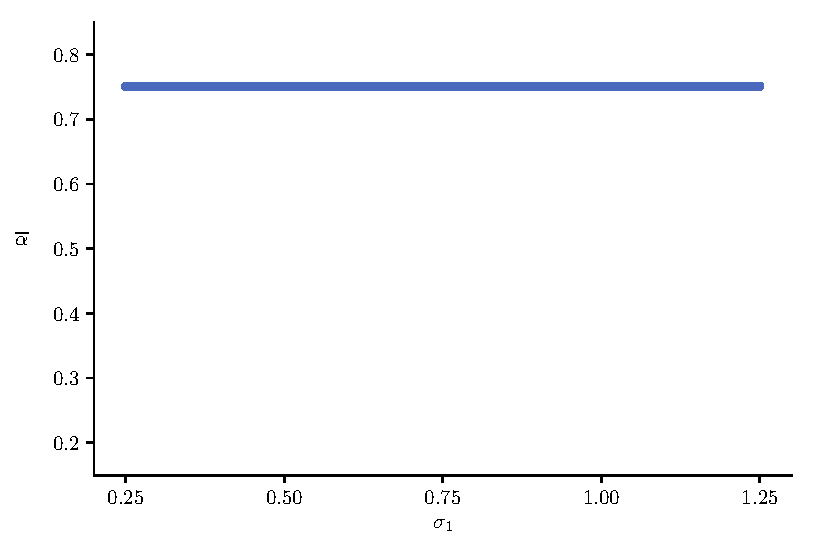
\includegraphics[width = 0.45\textwidth]{CategoryAlphasPlot_0} \label{fig:AlphaCata}}\hspace{0.02\textwidth}
		\subfloat[$\lambda = 1.5$]{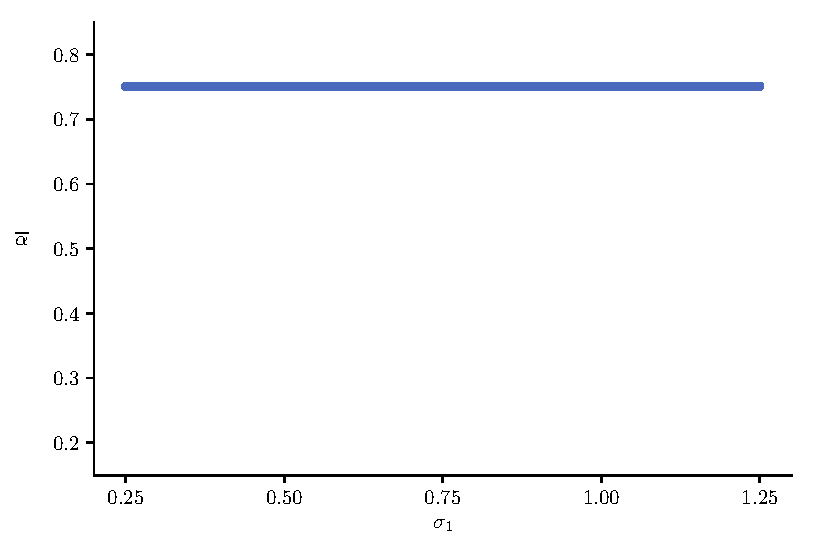
\includegraphics[width = 0.45\textwidth]{CategoryAlphasPlot_1} \label{fig:AlphaCatb}}
		
		\vspace{-1.5ex}
		\floatfoot{\begin{minipage}{0.95\textwidth}
			The blue line shows the optimal $\overline{\alpha}$ at $t = 1$ as a function of $\sigma_{1}$. Note that for $\sigma_{1} = 0$, the optimal value of $\overline{\alpha}$ is the same as the one computed at $t = 0$: $0.75$ (see \Cref{tab:OptimalAlphaT}). The price vectors used are $\mathbf{p}_{0} = (1,10)$ and $\mathbf{p}_{1} = \lambda_{i} \mathbf{p}_{0}$, with $i = 1,2$.
		\end{minipage}}
	\end{figure}


	


%%%%	Aggregation across goods	%%%
%\section{Aggregation across goods} \label{sec:OneGood}
%
%	%%	Economy setting	%%
%\subsection{Economy setting} \label{ssec:OneGoodDescr}
%Consider a two period economy with $n+1$ goods available, $(\mathbf{x}, z)$, valued at prices $(\mathbf{p}, q)$.  In what follows and for simplicity of notation, the subscripts $t$ for all variables are omitted unless needed. In this economy, consider one consumer whose income is $y \in (0,\infty)$.\footnote{\,I am not claiming there is only one consumer in the economy. Instead I am just focusing on one of them.} The vector $\alpha \in (0,1)^{n}$ determines the form of our consumer's pseudo-Cobb-Douglas (PCD) utility function,
%	$$u_{\alpha}(\mathbf{x},z) := u_{(y,\alpha)}(\mathbf{x},z) = \sum_{j=1}^{n} x_{j}^{\alpha_{j}}z^{1-\alpha_{j}}.$$
%
%Hence, the agent can be identified with the pair $(y,\alpha)$. This consumer chooses how much of the $\mathbf{x}$ goods to consume in each period according to
%	\begin{equation} \label{eq:probdisagg2}
%		\probop[s.t.]{\mathbf{x}(\mathbf{p}, q, y) 
%			:= \argmax_{\mathbf{x}, z}}{u_{\alpha}(\mathbf{x}, z),}
%				{&	\mathbf{p} \mathbf{x} + qz = y.}
%	\end{equation} 
%
%Observe that if all $\alpha_{j}$ are different, then it is not possible to bundle the $\mathbf{x}$ goods into a category. Indeed, as mentioned in \Cref{ssec:HicksAgg}, without assuming certain price dynamics, the only option is to be in presence of functional separability. A necessary condition for this to happen is that the $\mathbf{x}$ goods are independent of $z$ in terms of the preference, that is, \eqref{eq:indepPref} holds. It is straightforward to see that for the preference relation represented by the function $u_{\alpha}$ this property is not satisfied unless all $\alpha_{j}$ are equal. Furthermore, when $\alpha_{j} = \alpha_{0}$ for every $j$, aggregation is possible as was seen in \Cref{sec:MixedAgg}. 
%
%	%%	The estimation problem	%%
%\subsection{The estimation problem} \label{ssec:OneGoodProblem}
%An investigator at time $t=0$ is interested in studying the evolution of the demand on the $\mathbf{x}$ goods. For that purpose, instead of focusing in the individual demands on the $\mathbf{x}$ goods she wishes to construct a quantity index for them, $g_{\overline{\alpha}}$, like the one defined in \eqref{eq:qtyindex} in \Cref{ssec:RepAgDescr}. In other words, she wants to choose a value $\overline{\alpha}$ such that by defining $U$ and $P_{\overline{\alpha}}$ as in \eqref{eq:utilagg} and \eqref{eq:priceindex}, respectively, the category demand
%	\begin{equation} \label{eq:probagg2}
%		\probop[s.t.]{X(\mathbf{p}, q, y) := \argmax_{X, z}}{U(X,z)}
%										{&	P_{\overline{\alpha}}(\mathbf{p})X + qz = y,}
%	\end{equation}
%is the closest possible to $g_{\overline{\alpha}}(\mathbf{x}(\mathbf{p}),q,y)$. In general, the equality
%	$$X(\mathbf{p}, q, y) = g_{\overline{\alpha}}\big(\mathbf{x}(\mathbf{p}, q, y)\big),$$
%will not hold as was discussed in the previous section, but the choice of $\overline{\alpha}$ can be made optimally to reduce the difference as much as the researcher wants.
%
%Following the discussion in the previous sections, the question that arises in this setting is: Which heterogeneity is being approximated by assuming there is only two, instead of $n+1$ goods in the economy. The answer is straightforward and follows the same argumentative line. Since $\overline{\alpha}$ is replacing every $\alpha_{j}$ with a single parameter, then what is being approximated is the distribution of the $\alpha_{j}$, that is, the differences in preferences between the available goods. To see this, we can regard the heterogeneous preferences between the $\mathbf{x}$ goods as an equiprobable distribution with mass at each $\alpha_{j}$. This way of seeing this approximation is coherent with the previous examples where the distributions were representing the heterogeneity of the context, in particular the different preferences between individuals in the economy.
%
%	%%	Measuring the error	%%
%\subsection{Measuring the error} \label{ssec:OneGoodError}


%%%	Concluding remarks		%%%
\section{Concluding remarks} \label{sec:Conclusion}

%:	Summary
The previous exercises and problems depict three situations where the inherent diversity of a model is replaced with a completely homogeneous alternative. In all three cases, aggregation is used as a tool to overcome the complexity imposed by differences between agents. This work diverges from previous attempts to study aggregate models not on the objective but on the means to attain it. In both there is a quest to obtain requisites that ensure coherence between homogeneous and heterogeneous models. However, while the latter seek to impose these requirements on the disaggregate model, I claim instead that a better approach is to introduce them on the aggregate one. The advantage of this alternative is that it suppress all restrictions about what kind of model can be subject to aggregation. As a consequence, all previous models that ignored the conditions to have exact aggregation can be now evaluated in terms of the quality of the fit, instead of the lack of the right context to apply it. In particular, this way of thinking the problem has implications on a variety of models where intrinsic differences are part of their essence.

%:	Abstracting the main idea
In broader terms, the main idea I present in this paper is that aggregation can be regarded as a tool or solution used in the problem of heterogeneity approximation. Following the insights and lines of argumentation of the previous sections, I can reformulate this modeling problem as follows. Diversity is, in formal terms, the presence of a non-trivial distribution $F$ over a given set of parameters in the economy. Thus, the question of finding a suitable substitute to it consists of two parts: 1) determine which aspects of $F$ are relevant to the specific objective of the model, and 2) establish an appropriate distance between distributions that allows the researcher to select the best $\hat{F}$ to replace $F$. This way, the original problem, which may be ambiguous in its conception, is replaced by one that is both transparent and susceptible to be tackled directly using mathematical tools.

%:	Part 1)
The first part of the question is equivalent to determining the most significant sources of heterogeneity and how to model them. For that reason, the result of this search is inevitably tied to the particular problem the researcher is trying to confront. However, this does not necessary imply that obtaining the answer is difficult. On the contrary, this phase of the modeling problem was already present and, moreover, is allegedly easier since heterogeneous features within a model are generally the fundamental part of the question. Nevertheless, it is clear that when finding the answer some decision about the extent of the disaggregate nature of the model has to be made. Indeed, note that the dual of the question asks which aspects of $F$ are not relevant and, consequently, not included in the approximation problem. An additional advantage is that reviewing the most important aspects of the problem at hand may give some hints regarding the next step: choosing the distance between distributions. By narrowing the sources of heterogeneity it is conceivable that an appropriate measure of error emerges naturally.

%:	Part 2)
The second stage of the question, adopting a suitable distance, is probably the hardest of the two. In optimization terms, the problem requires to carefully define the loss function to use. In the examples developed throughout this text the metrics used are simple differences between the real and estimated values of the variable of interest. This later implied that the error could be written in terms of a certain number moments of both the original and approximate distributions. Arguably, other types of loss functions can result in better alternative models if their choice is capable of correcting deficiencies that may arise when using the ones I introduced throughout the text. However, in the case of a researcher interested in a given variable (or set of variables) $X$, the simple-difference choice may be backed by the fact that for a certain tolerance in the goodness-of-fit, a Taylor approximation of $X$ around a previously know point (e.g., the known value at the moment of the modeling process) can be made. This polynomial provides the relevant moments of the variables that are needed to have a suitable fit. Therefore, a possibility is using another distribution $\hat{F}$ that shares those moments with $F$. Another option is using a simpler $\hat{F}$ that is calibrated using this same approximation, like the examples in the paper.

%:	Closing comments and future challenges
The above discussion makes clear that taking into account the full diversity of the model and using a completely aggregate one are two extremes of a wide spectrum of possibilities. Depending on the particular problem to confront, the most desirable approximation likely lies between the two. For the models I present in this work, the aggregate extreme is always a feasible solution, but it is not necessarily optimal under every criteria. Moreover, this analysis only takes care of problems where the interest is predicting an aggregate variable. This is the crucial feature that implies that the estimation differences depend on some unknown moments of the original distribution. Specific examples remain to be studied where the interest is of a different kind (e.g., estimation of treatment effects or robustness of the conclusions of a model). As mentioned before, it is plausible that the main challenge in any other modeling problem is the choice of the appropriate measure of error or, in other words, the distance between the chosen distributions. \rojo{All in all, these tasks provide am unifying framework for researchers that deal with problems in which diversity of any kind makes an appearance.}

\newpage
\section*{Acknowledgements}
The paper I developed in the preceding pages is the product of a process longer than the four months it took to write. Within each sentence my words bear a hidden meaning, a testament of the experiences I have been through.  They speak about education, at home, at school, at college. They represent dedication, responsibility, tenacity. But mostly they are a reflection of support. This work would have not be the same without the encouragement and company of many people I met from the earliest to this latest part of my life. To everyone of you, I dedicate this work.

To my parents. I start with you because that is how it all began. A great part of the success of this (long) journey has been without doubt a result of countless efforts from both. Thanks for your unconditional support, for the values and virtues you taught and showed me since my birth. Thank you for proving me that hard-work, patience and discipline are key to achieve any objective. Thank you for giving me the privilege of a good school and a top-notch education in general. Above all, I am grateful for your unquestioning love, your company and the luck to have you as parents. I wish this paper makes you proud.

To my grandmother, Miss Glory. It is impossible to imagine this moment without you. You have been an extraordinary company in every stage of the way and for that I am grateful. As a kid I was kind of your young side-kick but I think we are more like partners now. I sincerely hope you feel proud of me and that you think of this achievement as part of you too. With all my love, this thesis is for you. 

To my friends (in alphabetical order), Raúl, Iván, Pancho, David, Pato, Rubén, Nacho. Maybe you are not aware but your presence in my life was key to reach this moment. From early in school to these last days of college your company and encouragement have shaped me into the person who I am today. Thank you for that. It may sound trivial (pun intended) but having moments of leisure with you playing video games or just having a burger together at a birthday will be without doubt one of the most valuable memories I will cherish forever. Again and always, thank you.

To my guides, Felipe and Eugenio. I can not imagine how tiresome and difficult it must be to help a student to reach high quality academic work in such a short amount of time. You showed dedication up to the last minute in spite of the unexpected conditions at the end of the semester. Not only that, you proved patient when we were lost and out of focus. Thank you for all your work in this four months.

Last but not least, to Nine. \textit{Thank you} is not the word I'm looking for, there is so much more inside me now. It is evident that without you this thesis would have not been the document I feel proud of. Your comments were critical to reach this point. But your support does not even begin there. You enlightened the way when I thought I was writing nonsense. You encouraged me when I ran out of ideas. You were there just to hear me ranting when I needed. I love you for that, for your kindness, your intelligence and your dedication towards us. I feel the luckiest person in the world for finding the most wonderful teammate. I sincerely hope to be the partner you need me to be and to repay at least a drop of all the love you give me. G r a t i t u d e.

%: 	Bibliography
\bibliographystyle{abbrvnat}
\bibliography{GoFModels}

\end{document}